
\title{Применение метода суперкомпиляции для специализации реляционных программ}
\titlerunning{Суперкомпиляция реляционных программ}

\author{Куклина Мария}
\authorrunning{Куклина М.}

\tocauthor{Куклина М.}
\institute{Национальный исследовательский университет ИТМО\\
	\email{kuklina.md@gmail.com}}

\maketitle



% \documentclass[14pt, a4paper] {extarticle}



% % Обязательно переносить слова, чтобы соблюсти поля документа. Для
% % соблюдения полей можно пренебречь правилами для тех слов и
% % словосочетаний, о которых не знают словаря переносов (ruhyphen или
% % ruenhyph). Оно почему-то работает. Взято с:
% %
% %   http://www.latex-community.org/forum/viewtopic.php?p=70342#p70342
% %
% \tolerance 1414
% \hbadness 1414
% \emergencystretch 1.5em
% \hfuzz 0.3pt
% \widowpenalty=10000
% \vfuzz \hfuzz
% \raggedbottom

%%%%%%%%%%%%%%%%%%%%%%%%%
\lstdefinelanguage{MyLang}
{
  morekeywords={data},
  keywordstyle=\bfseries\color{black}
}

%\lstset{language=Haskell}
\lstset {
mathescape,
extendedchars=\true,
basicstyle=\ttfamily,
numberstyle=\ttfamily,
numbers=left,
stepnumber=1,
frame=single,
morekeywords={data, do, type, if, then, else, class, where, return}
}

%%%%%%%%%%%%%%%%%%%%%%%%%
\newcommand{\larrow}{\leftarrow}
\newcommand{\rarrow}{\rightarrow}

\newcommand{\embed}{\unlhd}
\newcommand{\instance}{\preccurlyeq}
\newcommand{\strictinst}{\prec}
% \newcommand{\variant}{\leftrightarrow}
\newcommand{\variant}{\approx}
\newcommand{\genup}{\lessdot}

\newcommand{\ukanren}{$\mu$Kanren }
\newcommand{\forcpd}{конъюнктивной частичной дедукции }
\newcommand{\cpd}{конъюнктивная частичная дедукция }
\newcommand{\Cpd}{Конъюнктивная частичная дедукция }

\newcommand{\origin}[1]{(англ. {\it #1})}

\newcommand{\relo}[1]{$\text{#1}^o$}

%%%%%%%%%%%%%%%%%%%%%%%%%

\graphicspath{{Kuklina/}}

% \addbibresource{main.bib}

% \begin{document}
\setcounter{figure}{0}
\setcounter{page}{4}
\section{Введение}
С каждым годом сложность программных продуктов возрастает, и, соответственно, задача обеспечения их надёжности и корректности становится всё более востребованной. Для её решения используются активно развивающиеся техники из области верификации. Одной из таких техник является символьное исполнение~\cite{wenenhancing, li2014symbolic}.

Некоторые современные верификаторы~\cite{sethu2018systems, wang2017dependence, sharma2018veritesting} используют технику символьного исполнения для сведения задачи анализа программного кода с неопределёнными входными данными к проверке выполнимости формул логики первого порядка. Для такой проверки чаще всего используются SMT-решатели (Satisfiabilty Modulo Theories). Данные инструменты позволяют определить, выполнима ли формула, записанная в поддерживаемых
решателями теориях (например, теория линейной арифметики, битовых векторов и некоторые другие). Таким образом в процессе сведения анализа программного кода к проверке выполнимости формул логики необходимо моделировать семантику программы в теориях логики первого порядка, поддерживаемых решателями.

В современных языках программирования, таких как \clang{}, \textsc{C++}, \textsc{C\#}, \textsc{Java} и других, память программы достаточно полно отражает состояние этой программы, и операции с памятью имеются почти в каждой нетривиальной программе. Соответственно, разработка метода моделирования операций с памятью для последующего использования в SMT-решателе является важной и актуальной задачей верификации. Метод моделирования операций с памятью (т. е. \emph{модель памяти}) определим, согласно статье~\cite{mandrik}, как формальное представление указателя и ссылки, а также формализацию результата операций над ними c использованием логических формул. Разработка такого метода позволила бы доказывать, что в программе, например, отсутствуют: утечки памяти, некорректные доступы к памяти (например, выход за границы массива), неопределённые поведения и т.д. Однако задача разработки модели памяти является нетривиальной, а её решение зависит от семантики конкретного языка программирования.

Важной особенностью платформы .NET является возможность использования динамической памяти, т.е. памяти заранее не ограниченного размера. Помимо этого в платформе .NET существует два контекста исполнения кода: безопасный (англ. safe) и небезопасный (англ. unsafe). В случае безопасного контекста, низкоуровневыми операциями с памятью управляет \textsc{CLR} (Common Language Runtime). Когда контекст исполнения является небезопасным, пользователю становятся доступны операции с указателями, как в языке \clang{}, которые могут привести к \emph{реинтерпретации данных}.

Под реинтерпретацией понимается рассмотрение данных при помощи структуры\footnote{в широком смысле, от слова <<структурированный>>}, отличной от той, которой они изначально задавались. Такого поведения можно добиться с помощью адресной арифметики и приведения типов указателей, например, прочитав массив из элементов типа \lstinline[language=csharp]{int} указателем с типом \lstinline[language=csharp]{byte*}.

В данной статье представлен метод моделирования операций с памятью платформы .NET в условиях безопасного и небезопасного контекста. Для его создания был проведён обзор существующих на данный момент моделей памяти.

\section{Обзор предметной области}

Одним из подходов к заданию принтеров являются принтер-комбинаторы.
В этой главе приведен обзор классических принтер-комбинаторов, а также
принтер-комбинаторов с дополнительным оператором \emph{выбора}, которые
в рамках данной работы использованы для реализации принтеров, задаваемых
с помощью шаблонов. Для решения проблем эффективности
комбинаторов с выбором в данной работе был использован подход BURS.
Апробация подхода задания принтеров с помощью шаблонов
была произведена для языка Java, для которого есть средства форматирования,
встроенные в IDE.

\subsection{Принтер-комбинаторы}

Базовыми принтер-комбинаторными библиотеками являются библиотеки
Джона Хьюза\cite{hughes} и Филиппа Вадлера\cite{wadler}, которые
представляют собой функциональную переработку алгоритма
Оппена\cite{oppen}.
Ограничимся рассмотрением библиотеки Вадлера, так как
библиотека Хьюза обладает теми же свойствами, которые принципиальны в контексте
данной работы.

В библиотеке ключевым типом является документ.
Он представляет сущность, которая потом может
быть переведена в строковое представление алгоритмом принтера.
Основные конструкторы для составления документа таковы:
\begin{itemize}
  \item атомарная строка, которая печатается как есть;
  \item \emph{разделитель};
  \item последовательная композиция двух документов;
  \item набор связанных документов.
\end{itemize}

Определяющей особенностью данного подхода является то, что все разделители
в рамках одного набора могут быть совместно заменены алгоритмом принтера
на пробельный символ или на перевод строки. Выбор для каждого набора разделителей
основывается на том, что вывод должен поместиться в заданную ширину,
используя минимальное число строк.

Основная проблема такого подхода заключается в его слабой выразительной силе.
Документы, построенные по синтаксическому дереву печатаемой программы,
обрабатываются слишком единообразно, что иногда приводит к нежелательному результату.
Пусть, к примеру, нужно напечатать программу на языке
Python\footnote{\cd{http://python.org}}.
Между последовательными операторами в случае их печати на одной строчке необходимо
добавить дополнительный разделитель (``;''), иначе программа станет некорректной
(см. рис.~\ref{fig:seqEx}). Однако, описанные принтер-комбинаторы не предоставляют
возможности задать такое поведение.
Кроме того, с помощью таких принтер-комбинаторов невозможно выразить разные проектные СК,
так как они всегда печатают текст в одном стиле, который жестко ``зашит'' в их код.

\begin{figure}[h!]
	\centering
	\null\hfill
	\subfloat[Корректный код]{
		\centering
    \makebox[.4\textwidth] {
		  \lstinputlisting[language=Python]{codes/pythonCode.py}
    }
	}
	\null\hfill
	\subfloat[Некорректный код]{
		\centering
    \makebox[.4\textwidth] {
	  	\lstinputlisting[language=Python]{codes/pythonCodeBad.py}
    }
	}
	\hfill\null
	\caption{Пример работы принтер-комбинаторов для языка Python}
  \label{fig:seqEx}	
\end{figure}

Более подробный обзор библиотек Хьюза и Вадлера представлен в \cite{myCoursePaper}.

Большинство принтер-комбинаторных библиотек\cite{
swierstraChitil, swierstra04, peytonJones, kiselyov, chitil}
являются развитиями работ Хьюза и Вадлера. Так, в отличие от базовых, среди
них есть реализации с линейной сложностью обработки документа от его размера и
\emph{online} алгоритмы, которые не требуют просмотра всего документа
для начала печати его текстового представления. Но все они обладают тем же
интерфейсом, а значит в них также неразрешимы задачи, в которых требуется
задавать варианты текстовых представлений, которые отличаются не только
пробелами и переводами строк.

\subsection{Принтер-комбинаторы с выбором}

Существенно от описанных выше отличаются библиотеки, предоставляющие в своем
интерфейсе комбинатор \emph{выбора}, который позволяет задавать для одного поддерева
принципиально разные варианты раскладок.
Так, в работах~\cite{jongeEveryOccasion, jongeReengine} используется
оператор \lstinline[language = Haskell]{ALT},
но алгоритм принтера устроен так, что среди двух альтернатив выбирается первая, если она
помещается в заданную ширину, и вторая --- иначе,
что не дает оптимальный результат на выходе.

Оптимальные принтер-комбинаторы с выбором были впервые представлены в работе~\cite{swierstra}.
Их реализация является частью Utrecht Tools
Library\footnote{\cd{http://www.cs.uu.nl/wiki/HUT/WebHome}}
(практическая реализация несколько изменена по
отношению к той, что описана в статье, но отличие несущественно).
В данном подходе текст строится из блоков прямоугольной формы с возможно неполной последней
строчкой (см. рис. \ref{fig:basicFormat}). В реализации на Haskell блоки представляются
структурой \lstinline[language = Haskell]{Format}:
\begin{lstlisting}
    data Format = Elem { height        :: Int
                       , lastLineWidth :: Int
                       , width         :: Int
                       , txtstr        :: Int -> String -> String
                       }
\end{lstlisting}

Первые три поля структуры определяют геометрические размеры блока, а последнее --- функция,
которая используется для преобразования блока в текст. Здесь используется функция, а не
просто строчка, чтобы можно было преобразовывать вложенные блоки за линейное время. Первый
аргумент \lstinline[language = Haskell]{txtstr} задает сдвиг блока.

\begin{figure}
  \centering
  \subfloat[Блок текста]{
    \raisebox{5mm}{
      \centering
      \vspace{0pt}
      \tikz[scale = 2.0]{
        \draw (0,0) -- (1,0) -- (1,0.2) -- (2,0.2) -- (2,1) -- (0, 1) -- cycle;
      }
    }
    \label{fig:basicFormat}
  }
  ~
  \subfloat[Горизонтальная композиция]{
    \centering
    \tikz[scale = 2.0]{
       \draw (0,0) -- (1,0) -- (1,0.2) -- (2,0.2) -- (2,1) -- (0, 1) -- cycle;
       \draw (1.1,-0.9) -- (2.1,-0.9) -- (2.1,-0.7) -- (3.1,-0.7) -- (3.1,0.1) -- (1.1,0.1) -- cycle;
     }
     \label{fig:beside}
  }
  %\hfill
  ~
  \subfloat[Вертикальная композиция]{
    \makebox[.28\textwidth] {
    \centering
    \tikz[scale = 2.0]{
       \draw (0,0) -- (1,0) -- (1,0.2) -- (2,0.2) -- (2,1) -- (0, 1) -- cycle;
       \draw (0,-1.1) -- (1,-1.1) -- (1,-0.9) -- (2,-0.9) -- (2,-0.1) -- (0,-0.1) -- cycle;
    }
    \label{fig:above}
    }
  }
  \caption{Примитивы блока текста}
  \label{fig:basicConcat}
\end{figure}

Для работы с блоками текста используется следующие четыре примитива:
\begin{lstlisting}
    s2fmt     :: String -> Format
    indentFmt :: Int -> Format -> Format
    aboveFmt  :: Format -> Format -> Format
    besideFmt :: Format -> Format -> Format
\end{lstlisting}

Функция \lstinline[language = Haskell]{s2fmt} создает блок текста,
состоящий из одной строчки; \lstinline[language = Haskell]{indentFmt} по блоку создает новый,
сдвинутый на заданное число позиций. Действие примитивов композиции
\lstinline[language = Haskell]{besideFmt} и \lstinline[language = Haskell]{aboveFmt}
показано на рис.~\ref{fig:beside} и \ref{fig:above} соответственно.

Также, как и в библиотеках без комбинатора выбора, в работе~\cite{swierstra} используется понятие
\emph{документа}. Здесь документ можно рассматривать как множество возможных раскладок
(набор \lstinline[language = Haskell]{Format}-элементов). Документы описываются типом
\lstinline[language = Haskell]{Doc}, экземпляры которого на этапе построения представляют собой
деревья применений приведенных ниже комбинаторов, а на этапе обработки алгоритмом
принтера им в соответствие ставится итоговое множество вариантов текстовых представлений.

Документ конструируется с помощью следующих комбинаторов, которые симметричны
примитивам построения блоков текста:
\begin{lstlisting}
    text   :: String -> Doc
    indent :: Int -> Doc -> Doc
    beside :: Doc -> Doc -> Doc
    above  :: Doc -> Doc -> Doc
\end{lstlisting}

В дополнение появляется пятый комбинатор для документов:
\begin{lstlisting}
    choice :: Doc -> Doc -> Doc
\end{lstlisting}

Этот комбинатор и является тем самым комбинатором выбора. Он представляет
\emph{объединение} множеств раскладок документов, которые были переданы как
аргументы комбинатора. Заметим, что только этот комбинатор может произвести
документ с несколькими раскладками из одновариантных аргументов.

Оригинальная реализация существенно опирается на ленивые вычисления. В \cite{swierstra}
множество вариантов, соответствующее экземпляру \lstinline[language = Haskell]{Doc},
представляется ленивым списком всех возможных раскладок, удовлетворяющих ограничению
на максимальную ширину. Этот список отсортирован в порядке ``ухудшения''
раскладок, то есть в голове списка лежит ``лучшая'', в терминах оптимальности,
раскладка из возможных при заданной ширине. В случае
\lstinline{beside}- и
\lstinline{above}-композиций
документов полная (без учета ленивости) сложность вычисления списка нового документа
составляет $O(n \times m)$, где $n$ и $m$ --- размеры списков, соответствующих 
соединяемым документам. Размер нового списка также порядка $n \times m$.
Он не обязательно точно равен $n \times m$, так как некоторые из полученных
представлений могут не подпадать под ограничение на ширину, соответственно их можно
отбросить на этапе построения нового списка.

Выбор лучшего представления для самого верхнеуровнего документа происходит
просто --- нужно из соответствующего списка взять первый элемент.
Это создает впечатление, что общее число операций,
благодаря ленивым вычислениям, существенно уменьшается.
Но это не так из-за реализации обработки документа,
построенного с помощью комбинатора \lstinline[language = Haskell]{beside}, которая
вынуждает полное вычисление дочерних списков. Более того, из-за свойств отношения
порядка, построенного по критерию оптимальности, в рамках данной модели списков
принципиально нельзя построить ленивую обработку комбинатора
\lstinline[language = Haskell]{beside}.
Так, выбор оптимальной раскладки документа в
\cite{swierstra} имеет в худшем случае экспоненциальную сложность от числа
комбинаторов, использованных при его построении.
В \cite{swiComb} приведены оптимизации для данной модели, но они
не улучшают асимптотику решения для деревьев в общем случае.

\subsection{BURS}

Bottom-Up Rewrite System (BURS)\cite{burs} --- это метод динамического
программирования на деревьях, изначально появившийся в контексте задачи выбора
инструкций для генерации машинного кода. Основой BURS является
регулярная грамматика с древовидными правилами\cite{tata}, для которых задана
стоимость применения подстановки,
то есть грамматика со следующим набором правил: 

$$
\begin{array}{rcll}
  N &:& \alpha& [c]\\
  N &:& \alpha\; (K_1,\dots,K_n)& [c]
\end{array}
$$

Здесь $N, K_i$ это нетерминалы, $\alpha$ --- терминал,
$c$ --- функция стоимости, заданная для каждого правила.
Как и для обычной линейной грамматики, вводится стартовый
нетерминал S. Считается, что терминальное дерево выводится в
данной грамматике, если его можно получить с помощью правил
подстановки из одноузлового дерева $S$.
Каждая подстановка заменяет нетерминал $N$, находящийся в листе дерева, на дерево 
$\alpha\;(K_1,\dots,K_n)$, если в грамматике есть правило
$N:\alpha\;(K_1,\dots,K_n)$. 
Для каждой подстановки вычисляется стоимость ее применения с помощью
функции стоимости $c$.
Аргументами функции могут служить терминальная метка $\alpha$ и стоимости
вывода поддеревьев.
Задачей, которую решает BURS, является поиск вывода наименьшей стоимости
для заданного дерева по заданной грамматике.
Такой вывод может быть найден двухпроходным алгоритмом.

Первый проход (\emph{пометка}) обрабатывает дерево снизу вверх и вычисляет
для каждого узла набор троек $(K,\;R,\;c)$, где $K$ --- нетерминал, из которого может быть
выведено поддерево с корнем в обрабатываемом узле,
$R$ --- первое правило, которое используется для вывода минимальной стоимости из $K$,
$c$ --- стоимость такого вывода.
Процесс пометки происходит следующим образом:

\begin{itemize}
\item для листовой вершины, помеченной терминалом $\alpha$, в множество троек
этого вершины добавляется $(K,\;R,\;c\:(\alpha))$ для каждого правила $R=K:\;\alpha\;[c]$;
\item для промежуточной вершины, помеченной терминалом $\alpha$,
с непосредственными поддеревьями $v_1,\dots,v_n$
в множество добавляется тройка $(K,\;R,\;c\:(\alpha,c_1,\dots,c_n))$ для каждого правила
$R=K:\;\alpha\;(K_1,\dots,K_n)\;[c]$, где $(K_i,\;R_i,\;c_i)$ входит в множество троек для
$v_i$; если есть несколько правил вывода из нетерминала $K$, то выбирается правило,
минимизирующее стоимость вывода.
\end{itemize}

Второй проход (\emph{свертка}) просматривает дерево сверху вниз, используя сделанные пометки.
Первое правило из минимального вывода определяется тройкой $(S,\;R,\;c)$ для корневого узла
(если такой тройки нет, то вывод из $S$ невозможен).
Это правило однозначно определяет нетерминалы $K_i$ для каждого непосредственного поддерева
и процесс повторяется.

Для пометки дерева потенциально необходимо каждое правило грамматики применить к каждому узлу.
При фиксированной грамматике алгоритмическая сложность первого прохода --- $O\:(|R|)$,
где $|R|$ --- количество правил
(размер множества троек для каждого узла ограничен числом нетерминалов, которое не больше,
чем количество правил). Свертка также имеет линейную сложность.


\newpage
\subsection{Средства форматирования кода в IDE}

Интегрированные среды разработки программного обеспечения
(IDE) предоставляют средства
для форматирования программного кода. Рассмотрим их на примере двух Java IDE ---
IntelliJ IDEA\footnote{\cd{http://jetbrains.com/idea/}} и
Eclipse\footnote{\cd{http://eclipse.org}}.
Для задания требуемого СК используется широкий набор настроек \emph{форматтера},
подпрограммы IDE, отвечающей за форматирование исходных текстов.
Примерами таких настроек являются:
\begin{itemize}
  \item помещать ли фигурную скобку на той же строке, что и
    предыдущее выражение;
  \item форматирование списков --- всегда на одной строчке, переводить строчку после
    каждого элемента или печатать на одной строке,
    пока строчка меньше заданной рекомендуемой ширины.
%   \item и т.д.
\end{itemize}
На рис. ~\ref{fig:ideaFormatter} и~\ref{fig:eclipseFormatter} приведены диалоги задания
параметров форматирования в IntelliJ IDEA и Eclipse соответственно.

\begin{figure}[p]
	\centering
	\includegraphics[width=\textwidth]{ideaFormatter}
	\caption{Окно настройки форматтера IntelliJ IDEA}
	\label{fig:ideaFormatter}
\end{figure}

\begin{figure}[p]
	\centering
	\includegraphics[width=\textwidth]{eclipseFormatter}
	\caption{Окно настройки форматтера Eclipse}
	\label{fig:eclipseFormatter}
\end{figure}

У встроенных форматтеров есть следующие особенности.
Во-первых, это невозможность выразить
нестандартный СК, так как настройки форматтеров, несмотря на их большое
количество,
дают ограниченную вариативность для текстовых представлений форматируемых
программ. В целом, количество принципиально разных
стилей форматирования, которые можно задать с помощью данных настроек,
невелико.
Во-вторых, в случае, если надо
придерживаться СК уже существующего проекта, то по коду этого проекта необходимо
вручную задать все настройки форматтера.
Причем наборы настроек в разных IDE не совпадают, что увеличивает сложность
поддержки единого СК, если разработчики используют отличные от друг друга IDE.
Для решения данной проблемы существуют плагины, позволяющие использовать
внешние фоматтеры\footnote{\cd{http://plugins.jetbrains.com/plugin/6546}}.
Кроме того, есть средства, позволяющие экспортировать настройки форматтера в
XML-файл для их использования в другой
IDE\footnote{\cd{http://blog.jetbrains.com/idea/2014/01/intellij-idea-13-importing-code-formatter-settings-from-eclipse/}}.

Важным достоинством описанных форматтеров является малое время работы.
Это достигается в том числе и за счет того, что часто форматируется не весь
файл, а только его часть (см. \cite{eclipse}),
и из-за детерминированности представлений узлов синтаксического дерева,
которая следует из специфики настроек форматтера.
Однако форматирование целого большого проекта занимает существенное время.
Например, обработка кода IntelliJ IDEA Community Edition занимает более часа
у встроенного в IDEA форматтера.


\section{Имеющиеся наработки}

В этом разделе описывается более подробно метод суперкомпиляции,
а также библиотека для специализации miniKanren, на основе
которой велась разработка.

\subsection{Алгоритмы cуперкомпиляции}

{\bf Суперкомпиляция} --- метод анализа и преобразования программ,
который отслеживает обобщённую возможную историю вычислений исходной
программы и строит на её основе эквивалентную ему, более оптимальную программу.
Впервые метод был предложен в работе~\cite{turchinSC}.

Упрощение достигается путём удаления или преобразования
некоторых избыточных действий: удаление лишнего кода, выполнение
операций над уже известными данными, избавление от промежуточных
структур данных, инлайнинг, превращение многопроходного алгоритма
в однопроходный и другие~\cite{scompRevisited}.
Также cуперкомпиляция может применяться для специализации программ.

% В конечном счёте, суперкомпилятор может придать программе линейное ускорение

Суперкомпиляция включает в себя частичные вычисления, однако не
сводится к ним полностью и может привести в глубоким структурным
изменениям оригинальной программы.

Суперкомпиляторы, которые используют только ``положительную''
информацию --- то есть информацию о том, что свободные переменные
чему-то равны, --- называют
позитивными~\origin{positive supercompilation}~\cite{scPos}.
К примеру, при достижении условного выражения
{\bf if} x $=$ a {\bf then} $t_1$ {\bf else} $t_2$
позитивный суперкомпилятор при вычислении $t_1$ будет учитывать то,
что x $=$ a, однако при вычислении $t_2$ он не будет знать, что
x $\neq$ a.
Расширение позитивного компилятора c поддержкой такой ``негативной''
информации --- идеальный
суперкомпилятор~\origin{perfect supercompilation}~\cite{scPerf}.

Техника суперкомпиляции в основном применяется для
функциональных~\cite{scHaskell, scPos} и императивных~\cite{scJava}
языков.
Для логических языков суперкомпиляция слабо развита, однако существует
посвящённые ей работы:
в работе~\cite{pdAndDriving} демонстрируется схожесть подходов частичной дедукции
и суперкомпиляции,
в работе~\cite{apropos} представлен позитивный суперкомпилятор APROPOS
для Prolog, однако эта версия довольно ограничена в своих возможностях
и требует ручного вмешательства.

%\todo{Кажется, нужны какие-то выводы}

% Общая схема суперкомпилятора представлена на рисунке~\ref{fig:scompScheme}
% \begin{figure}
% \center
% \includegraphics[scale=0.8]{./review/scompflow.pdf}
% \caption{Общая схема суперкомпилятора.}
% \label{fig:scompScheme}
% \end{figure}


% История вычислений при суперкомпиляции представляется в виде \emph{графа процессов} --- корневого ориентированного графа,
% в котором каждая ветвь --- это отдельный путь вычислений, а каждый узел --- состояние системы или \emph{конфигурация}.
% Конфигурация обобщённо описывает множество состояний вычислительной системы или её подсистемы.
% К примеру, конфигурацией можно назвать выражение $1 + x$, в котором параметр $x$ пробегает
% все возможные значения своего домена (допустим, множество натуральных чисел) и задаёт
% таким образом множество состояний программы\cite{turchinSC}.

% Процесс построение графа процессов называется \emph{прогонкой}~\origin{driving}.
% Во время прогонки производится шаг символьных вычислений, после которого
% в граф процессов добавляются порождённые конфигурации; множество конфигураций
% появляется тогда, когда ветвления в программе зависят от свободных переменных.

% В процессе прогонки в конфигурациях могут появляться новые свободные переменные,
% которые строятся из исходной конфигурации:
% если при вычислении выражения его переменная перешла в другую переменную (к примеру, из-за сопоставления с образцом),
% то в итоговую конфигурацию будет подставлена новая переменная и связь старой и новой сохранится в
% некоторой \emph{подстановке}.
% Подстановка --- это отображение из множества переменных в множество возможно замкнутых термов.
% Применение подстановки к выражению заменит все вхождения переменных, принадлежащих её домену,
% на соответствующие термы. %\todo{Что-нибудь ещё}

% Пример графа процессов представлен на рисунке~\ref{fig:pgraphExample}.
% \begin{figure}[h!]
% \center
% \begin{tikzpicture}[->,node distance=3cm, sibling distance=5cm]
                                                            
%   \tikzstyle{conf}=[rectangle,draw, rounded corners=.8ex]

%   \node[conf] (root) {$(a + b) + c$} ;
%   \node[conf] (childLeft) [below left of = root] {$b + c$};
%   \node[conf] (childRight)[below right of = root] {$(\text{Succ}(a_1) + b) + c$};
%   \path (root) edge node[above left,pos=1] {$\{a \mapsto \text{Zero}\}$} (childLeft)
%         (root) edge node[above right,pos=1]{$\{a \mapsto \text{Succ}(a_1)\}$}(childRight);
% \end{tikzpicture}

% \caption{Пример части графа процессов.}
% \label{fig:pgraphExample}
% \end{figure}
% Здесь при исполнении выражение $(a + b) + c$, где $a, b, c$ -- натуральные числа,
% были рассмотрены возможные значения $a$: это либо оно равно нулю (конструктор Zero), либо это некоторое
% число $a_1$, которому прибавили единицу (конструктор Succ). Эти два случая могут задают
% различные пути исполнения и, соответственно, добавлены в дерево процессов как два различных состояния,
% в одно из которых войдёт программа при исполнении.



% Потенциально процесс прогонки бесконечный, к примеру, когда происходят рекурсивные вызовы.
% Для превращения бесконечого дерева вычисления в конечный объект, по которому множно
% восстановить исходное дерево, используется \emph{свёртка.}

% Свёртка~\origin{folding}~--- это процесс преобразования дерева процессов в граф, при котором
% из вершины $v_c$ добавляется ребро в родительскую вершину $v_p$,
% если выражение в конфигурации в $v_c$ и в $v_p$ равны с точностью до переименования.
% Пример ситуации для свёртки изображён на рисунке~\ref{fig:pgraphFoldingExample},
% на котором свёрточное ребро изображено пунктиром.

% \begin{figure}[h!]
% \center
% \begin{tikzpicture}[->,node distance=2.3cm, sibling distance=5cm]
                                                            
%   \tikzstyle{conf}=[rectangle,draw, rounded corners=.8ex]

%   \node[conf] (root) {$a + b$} ;
%   \node[conf] (childLeft) [below left of = root] {$b$};
%   \node[conf] (childRight)[below right of = root] {$(\text{Succ}(a_1) + b)$};
%   \node[conf] (childRight2)[below  of = childRight] {$(a_1 + b)$};
%   \node (left)[below of = childLeft] {$\cdots$};

%   \path (root) edge node[above left,pos=1] {$\{a \mapsto \text{Zero}\}$} (childLeft)
%         (root) edge node[above right,pos=1]{$\{a \mapsto \text{Succ}(a_1)\}$}(childRight)
%         (childLeft) edge (left)
%         (childRight) edge (childRight2)
%         (childRight2) edge[bend right=90] (root);
% \end{tikzpicture}

% \caption{Пример свёртки. \todo{сделать соответствующим описанию в тексте.}}
% \label{fig:pgraphFoldingExample}
% \end{figure}

% Однако существует ситуации, при котором свёртка не приведёт к тому, что граф превратится в
% конечный объект. Такое может произойти, к примеру, когда два выражения структурно
% схожи, но не существует переименования, уравнивающих их: $a + b$ и $a + a$.

% Для решения этой проблемы используется \emph{обобщение}\cite{scGen}. Обобщение --- это процесс
% замены одной конфигурации на другую, более абстрактную, описывающую больше состояний
% программы. Для обнаружения ``похожей'' конфигурации используется предикат,
% традиционно называемый \emph{свистком}: свисток пробегает по всем
% родителям текущей конфигурации и определяет, похожа ли конфигурация на кого-то из них.
% В случае, когда свисток сигнализирует о найденной схожести, применяется обобщение.
% Сам шаг обобщения может произвести действия трёх видов:
% \begin{itemize}
% \item \emph{обобщение вниз} приводит к тому, что новая конфигурация заменяет текущую в графе процессов;
% \item \emph{обобщение вверх} приводит к замене родительской конфигурации на обобщённую;
% \item \emph{разделение}~\origin{split} используется для декомпозиции выражении, элементы которого затем
% будут обработаны отдельно.
% \end{itemize}
% Пример обобщения представлен на рисунке~\ref{fig:pgraphGenExample}

% \begin{figure}[h!]
% \includegraphics[scale=0.3]{./review/scgenex_temp.png}
% \caption{Пример обобщения \todo{свой рисунок}.}
% \label{fig:pgraphGenExample}
% \end{figure}

% Построение программы по графу конфигураций называется \emph{резидуализацией}, а
% построенная программа --- \emph{остаточной} \origin{residual}.
% Алгоритм выявления остаточной программы основан на обходе дерева, но
% в остальном полностью зависит от языка.

% \todo{Написать ещё про СК; продемонстрировать результаты СК; выводы}


\subsection{Язык \ukanren}

В данной работе для специализации был выбран \ukanren --- минималистичный диалект языка miniKanren~\cite{uKanren}.
\ukanren содержит только чистые операторы, что значительно упрощает процесс специализации.

Абстрактный синтаксис языка представлен на Рисунке~\ref{fig:syntax}.

\begin{figure}[h!]
\centering
\[\begin{array}{ccll}
  \mathcal{C}   & = & \{C_i\}                                                   &\mbox{конструктор с арностью}\ i \\
  \mathcal{X}   & = & \{ x, y, z, \dots \}                                      &\mbox{переменные} \\
  \mathcal{T}_X & = & X \cup \{C_i (t_1, \dots, t_i) \mid t_j\in\mathcal{T}_X\} &\mbox{термы над множеством переменных} \\
  \mathcal{D}   & = & \mathcal{T}_\emptyset                                     &\mbox{замкнутое выражение}\\
  \mathcal{R}   & = & \{ R_i\}                                                  &\mbox{реляционный символ с арностью}\ i \\[2mm]
  \mathcal{G}   & = & \mathcal{T_X}\equiv\mathcal{T_X}                          &\mbox{унификация} \\
                &   & \mathcal{G}\land\mathcal{G}                               &\mbox{конъюнкция} \\
                &   & \mathcal{G}\lor\mathcal{G}                                &\mbox{дизъюнкция} \\
                &   & \mbox{\lstinline|fresh|}\;\mathcal{X}\;.\;\mathcal{G}     &\mbox{введение свежей переменной} \\
                &   & R_i (t_1,\dots,t_i),\;t_j\in\mathcal{T_X}                 &\mbox{вызов отношения} \\[2mm]
  \mathcal{S}   & = & \{R_i^j = \lambda\;x_1\dots x_i\,.\, g_j;\}\; g           &\mbox{спецификация программы}
\end{array}\]
\caption{Синтаксис языка \ukanren~\cite{semanticMK}.}
\label{fig:syntax}
\end{figure}

\begin{itemize}
\item Унификация двух термов $t_1 \equiv t_2$ порождает подстановку $\theta$, называемую \emph{унификатором},
      такую что её применение к термам уравнивает их: $t_1 \theta = t_2 \theta$.

      Алгоритм унификации языков семейства miniKanren использует проверку вхождения \origin{occurs check},
      что гарантирует корректность получаемых унификаторов, однако довольно сильно замедляет выполнение программ.

\item Конъюнкция двух целей $g_1 \land g_2$ подразумевает одновременное успешное выполнение выражений $g_1$ и $g_2$.
\item Дизъюнкция двух целей $g_1 \lor g_2$ подразумевает, что достаточно, чтобы хотя бы одно из выражений $g_1$ или $g_2$ выполнялось успешно.
      Следует отметить, что при выполнении $g_1$ выражение $g_2$ также будет вычисляться.
\item Введение свежей переменной \lstinline{fresh} в языках miniKanren нужно указывать явно, в отличие, к примеру,
      от Prolog, где это происходит неявно.
\item Вызов реляционного отношения приводит к тому, что переданные в отношение термы
      унифицируются с аргументами отношения и подставляются в тело отношения. 
\end{itemize}

В контексте вычислений важно различие между \emph{синтаксическими} переменными, которые
определяются в тексте программы и обычно представляются строковыми литералами, и
\emph{семантическими} переменными, которые непосредственно используются в процессе вычислений и
представляются целыми числами, с которыми легче работать и генерировать свежие.

\ukanren является ядром языка miniKanren и может быть без труда расширен необходимыми
конструкциями.


\subsection{Библиотека для специализации miniKanren}

Реализация суперкомпилятора для \ukanren строилась на основе проекта по специализации \ukanren с помощью конъюнктивной частичной
дедукции\footnote{Проект \url{https://github.com/kajigor/uKanren_transformations/}, дата последнего посещения: 10.05.2020} на функциональном языке программирования Haskell.
Результаты специализации \ukanren представлены в работе~\cite{lozov}.

Библиотека вводит ряд структур данных и алгоритмов для реализации конъюнктивной частичной дедукции,
однако существует возможность её переиспользования для суперкомпиляции в силу нескольких доводов:
\begin{itemize}
\item схожесть методов частичной дедукции и суперкомпиляции~\cite{pdAndDriving},
      из чего следует, что ряд вспомогательных функций и определений и для частичной дедукции, и для суперкомпиляции
      будут совпадать;
\item алгоритм обобщения конъюнктивной частичной дедукции~\cite{cpd}, о котором подробнее будет рассказано позже,
      имеет ряд общих черт с процессом обобщения в суперкомпиляции;
\item библиотека предоставляет возможность преобразования сгенерированной программы
      на miniKanren, при котором удаляются излишние унификации и
      происходит удаление лишних аргументов~\origin{redundant argument filtering}~\cite{raf},
      что приводит в увеличению производительности программы, поскольку унификация --- операция дорогая.
\end{itemize}

В библиотеке введены структуры данных, описывающие термы и выражения языка
в соответствии с синтаксисом \ukanren на рисунке~\ref{fig:syntax}.
Над ними введён ряд важных структур и алгоритмов, речь о которых пойдёт ниже.
Основные операции над выражениями в конъюнктивной частичной дедукции производятся над конъюнкциями
%\emph{атомов}, --- то есть неделимыми элементами, которыми в miniKanren являются
вызовов реляционных отношений.

%%%%%%%%%%%%%%%%%%%%%%%%%%%%%%%%%%%%%%%%%%%%%%%%%%%%%%%%%
%%%%%%%%%%%%%%%%%%%%%%%%%%%%%%%%%%%%%%%%%%%%%%%%%%%%%%%%%
% Унификация
%%%%%%%%%%%%%%%%%%%%%%%%%%%%%%%%%%%%%%%%%%%%%%%%%%%%%%%%%
%%%%%%%%%%%%%%%%%%%%%%%%%%%%%%%%%%%%%%%%%%%%%%%%%%%%%%%%%

Во-первых, в библиотеке реализован алгоритм унификации двух термов.
Операция унификации находит наиболее общий унификатор \origin{most general unifier},
причём единственный, то есть такой
унификатор $\theta$, что для любого другого унификатора $\theta'$ существует подстановка $\sigma$,
с которой композиция наиболее общего унификатора даёт $\theta'$: $\theta' = \sigma \circ \theta$~\cite{unification}.
К примеру, для двух термов $f(X, 2)$ и $f(1, Y)$ наиболее общим унификатором является
подстановка $\{ X \mapsto 1, Y \mapsto 2 \}$, когда подстановки вроде
$\{ X \mapsto 1, Y \mapsto Z, Z \mapsto 2 \}$ также унифицирует термы, однако
содержат в себе лишние элементы.
Поиск наиболее общего унификатора уменьшает размер итоговой подстановки и является предпочтительным.

%%%%%%%%%%%%%%%%%%%%%%%%%%%%%%%%%%%%%%%%%%%%%%%%%%%%%%%%%
%%%%%%%%%%%%%%%%%%%%%%%%%%%%%%%%%%%%%%%%%%%%%%%%%%%%%%%%%
% Инстанс и вариант
%%%%%%%%%%%%%%%%%%%%%%%%%%%%%%%%%%%%%%%%%%%%%%%%%%%%%%%%%
%%%%%%%%%%%%%%%%%%%%%%%%%%%%%%%%%%%%%%%%%%%%%%%%%%%%%%%%%

Во-вторых, реализованы предикаты над термами, которые проясняют описанные ниже возможные связи термов.
\begin{itemize}
\item Выражение $e_2$ является \emph{экземпляром} выражения $e_1$ ($e_1 \instance e_2$),
если существует такая подстановка $\theta$, применение которой приравнивает
два выражения $e_1 \theta = e_2$; также говорят, что $e_1$ более общий, чем $e_2$.
К примеру, $f(X, Y) \instance f(Y, X)$. %и $f(X, Y) \instance f(Y, X)$ .
\item Выражение $e_2$ является \emph{строгим} экземпляром выражения $e_1$ ($e_1 \strictinst e_2$), если
$e_1 \instance e_2$ и $e_2 \not\instance e_1$. К примеру, $f(X, X) \strictinst f(X, Y)$, но не наоборот.
\item Выражения $e_1$ и $e_2$ \emph{варианты} друг друга $e_1\variant e_2$, если они являются экземплярами друг друга.
\end{itemize}

Предикат над вариантами определяет, являются ли два терма переименованием друг друга,
и поэтому может быть использован для свёртки графа процессов. Предикаты над экземплярами определяют
схожесть термов и используется в обобщении и в алгоритмах суперкомпиляции~\cite{scPos}.

%%%%%%%%%%%%%%%%%%%%%%%%%%%%%%%%%%%%%%%%%%%%%%%%%%%%%%%%%
%%%%%%%%%%%%%%%%%%%%%%%%%%%%%%%%%%%%%%%%%%%%%%%%%%%%%%%%%
% Свисток и гомеоморфное вложение
%%%%%%%%%%%%%%%%%%%%%%%%%%%%%%%%%%%%%%%%%%%%%%%%%%%%%%%%%
%%%%%%%%%%%%%%%%%%%%%%%%%%%%%%%%%%%%%%%%%%%%%%%%%%%%%%%%%

В-третьих, в качестве свистка используется отношение \emph{гомеоморфного вложения}~\cite{scGen}.
Отношение гомеоморфного вложения $\unlhd$ определено индуктивно:
\begin{itemize}
\item переменные вложены в переменные: $x \embed y$;
\item терм $X$ вложен в конструктор с именем $C$, если он вложен в один из аргументов конструктора:
      $$X \embed C_n(Y_1, \dots, Y_n): \exists i, X \embed Y_i;$$
\item конструкторы с одинаковыми именами состоят в отношении вложения, если в этом отношении
      состоят их аргументы:
      $$C_n(X_1, \dots, X_n) \embed C_n(Y_1, \dots, Y_n): \forall i, X_i \embed Y_i.$$
\end{itemize}

К примеру, выражение $c(b) \embed c(f(b))$, но $f(c(b)) \cancel{\embed} c(f(b))$.

Преимущество использования гомеоморфного вложения, в первую очередь, состоит в том,
что для этого отношения доказано, что на бесконечной последовательности выражений $e_0, e_1, \dots, e_n$
обязательно найдутся такие два индекса $i < j$, что $e_i \embed e_j$, вне зависимости
от того, каким образом последовательность выражений была получена~\cite{scPos}.
Это свойство позволяет доказать завершаемость алгоритма суперкомпиляции.

Однако отношение гомеоморфного вложения допускает, чтобы термы $f(X, X)$ и $f(X, Y)$
находились в отношении  $f(X, X) \embed f(X, Y)$ в силу того,
что все переменные вкладываются друг в друга. Однако обобщение
$f(X, X)$ и $f(X, Y)$ не привело бы к более общей конфигурации.

Отношение \emph{строгого} гомеоморфного вложения $\embed^+$ вводит дополнительное
требование, чтобы терм $X$, состоящий в отношении с $Y$, не был \emph{строгим экземпляром} $Y$~\cite{homeo}.
В таком случае отношение $f(X, X) \cancel{\embed}^+ f(X, Y)$, поскольку $f(X, Y)$ является строгим
экземпляром $f(X, X)$ из-за того, что существует подстановка $\{ X = X, Y = X \}$.

В рамках конъюнктивной частичной дедукции понятие гомеоморфного вложение было расширено на конъюнкции выражений.
Пусть $Q = A_1 \land \dots \land A_n$ и $Q'$ --- конъюнкции термов, тогда $Q \embed Q'$, тогда и только тогда,
когда $Q' \not\strictinst Q$ и существует упорядоченные подконъюнкции $A_1' \land \dots \land A_n'$
конъюнкции $Q'$, такие что $A_i \embed A_i'$~\cite{cpd}.
Конъюнкция $Q'$ может содержать в себе больше выражений за счёт того, что в этом случае при обобщении
произойдёт шаг разделения. Это расширение было реализовано в рассматриваемой библиотеке.

%%%%%%%%%%%%%%%%%%%%%%%%%%%%%%%%%%%%%%%%%%%%%%%%%%%%%%%%%
%%%%%%%%%%%%%%%%%%%%%%%%%%%%%%%%%%%%%%%%%%%%%%%%%%%%%%%%%
% Обобщение
%%%%%%%%%%%%%%%%%%%%%%%%%%%%%%%%%%%%%%%%%%%%%%%%%%%%%%%%%
%%%%%%%%%%%%%%%%%%%%%%%%%%%%%%%%%%%%%%%%%%%%%%%%%%%%%%%%%


В-четвёртых, реализован алгоритм обобщения для конъюнктивной частичной дедукции.
В общем, алгоритмы обобщения основаны на понятии \emph{наиболее тесного обобщения}.
\begin{itemize}
\item \emph{Обобщение} выражения $e_1$ и $e_2$ --- это выражение $e_g$, такое что
$e_g \instance e_1$  и $e_g \instance e_2$. На пример, обобщением выражения
$f(1, Y)$ и $f(X, 2)$ является $f(X, Y)$.
\item Наиболее тесное обобщение \origin{most specific generalization}
выражений $e_1$ и $e_2$ --- это обобщение $e_g$, такое что
для каждого обобщения $e_g' \instance e_1$ и $e_g' \instance e_2$ выполняется $e_g' \instance e_g$~\cite{scPos}.
Функция обобщения принимает на себя два терма $t_1$ и $t_2$ и возвращает
тройку $(t_g, \theta_1, \theta_2)$, такую что $t_1 \theta_1 = t_g$ и $t_2 \theta_2 = t_g$,
при этом $\theta_1$ и $\theta_2$ назовём \emph{обобщающими унификаторами} \origin{generalizers}.
\end{itemize}

% Алгоритм обобщения для конъюнктивной частичной дедукции, в соответствии со своим
% определением гомеоморфного вложения, выберет предка $Q^p$ для конъюнкции $Q$,
% такого что $Q^p \embed^+ Q$, и
% \todo{понять, как это доступно описать.}
Алгоритм обобщения для конъюнктивной частичной дедукции согласован с
определением гомеоморфного вложения
и используется в рамках \forcpd для построения более сложных алгоритмов обобщения,
свойственных методам частичной дедукции.
Однако его можно использовать как самостоятельный алгоритм для
суперкомпиляции, который соединяет в себе возможность произвести шаги обобщения
и разделения вместе, не выделяя отдельные шаги для это в процессе прогонки.


\subsection{Обобщённый алгоритм суперкомпиляции}

%%%%%%%%%%%%%%%%%%%%%%%%%%%%%%%%%%%%%%%%%%%%%%%%%%%%%%%%%%%%%%%%%%%
%%%%%%%%%%%%%%%%%%%%%%%%%%%%%%%%%%%%%%%%%%%%%%%%%%%%%%%%%%%%%%%%%%%
% Описание общего алгоритма суперкомпиляции
%%%%%%%%%%%%%%%%%%%%%%%%%%%%%%%%%%%%%%%%%%%%%%%%%%%%%%%%%%%%%%%%%%%
%%%%%%%%%%%%%%%%%%%%%%%%%%%%%%%%%%%%%%%%%%%%%%%%%%%%%%%%%%%%%%%%%%%

% На основе введёных выше терминов и операторов можно составить обобщённый алгоритм
% суперкомпиляции, который не затрагивает особенности и трудности реализации на Haskell.
% % Однако прежде необходимо ввести ряд необходимых понятий.

% %%%%%%%%%%%%%%%%%%%%%%%%%%%%%%%%%%%%%%%%%%%%%%%%%%%%%%%%%%%%%%%%%%%%
% %%%%%%%%%%%%%%%%%%%%%%%%%%%%%%%%%%%%%%%%%%%%%%%%%%%%%%%%%%%%%%%%%%%%
% %% Описание окружения
% %%%%%%%%%%%%%%%%%%%%%%%%%%%%%%%%%%%%%%%%%%%%%%%%%%%%%%%%%%%%%%%%%%%%
% %%%%%%%%%%%%%%%%%%%%%%%%%%%%%%%%%%%%%%%%%%%%%%%%%%%%%%%%%%%%%%%%%%%%
% %
% %\emph{Окружение} для суперкомпиляции должно сохранять следующие объекты:
% %\begin{itemize}
% %\item подстановку, в которой содержатся все накопленные непротиворечивые унификации,
% %      необходимую в процессе прогонки для проверки новых унификаций;
% %\item первую свободную семантическую переменную, необходимую для генерации свежих переменных,
% %      к примеру, при абстракции;
% %\item определение программы, необходимое для замены вызова на своё тело.
% %\end{itemize}
% % 
% % \todo{Что-то ещё об этом нужно написать!}

% Обобщённый алгоритм суперкомпиляции в псевдокоде представлен на рисунке~\ref{fig:scalgogen}.

% \begin{figure}[h!]
% % обобщение вверх
% % else if $\exists$ parent: parent $\genup$ configuration
% % then
% %    node $\larrow$ generalize(configuration, parent)
% %    addUp(env, tree, parent, node)

% \begin{lstlisting}[escapechar=@]
% supercomp(program, query):
%   env $\larrow$ createEnv program
%   configuration $\larrow$ initialize query
%   graph $\larrow$ emptyTree
%   drive(env, graph, configuration)
%   return residualize graph

% drive(env, graph, configuration):
%   if configuration is empty  @\label{line:success}@
%   then add(env, graph, success node)
%   else if $\exists$ parent: configuration $\variant$ parent @\label{line:renaming}@
%   then add(env, graph, renaming node)
%   else if $\exists$ parent: parent $\embed^+$ configuration @\label{line:abstraction}@
%   then
%     add(env, graph, abstraction node)
%     children $\larrow$ generalize(configuration, parent) @\label{line:gen}@
%     $\forall \text{child} \in \text{children}:$
%       drive(env, graph, child)
%   else @\label{line:unfolding}@
%     add(env, graph, unfolding node)
%     children $\larrow$ unfold(env, configuration) @\label{line:unfold}@
%     $\forall \text{child} \in \text{children}:$
%       drive(env, graph, child)
% \end{lstlisting}
% \caption{Обобщённый алгоритм суперкомпиляции.}
% \label{fig:scalgogen}
% \end{figure}

% Алгоритм суперкомпиляции принимает на себя программу и запрос,
% на который необходимо специализировать программу, и после
% инициализации начальных значений, включающих в себя некоторое \emph{окружения программы},
% в котором хранятся все вспомогательные структуры, запускает процесс прогонки.
% Прогонка производится до схождения и производит следующие действия в
% зависимости от состояния:
% \begin{itemize}
% \item если конфигурация пустая (строка~\ref{line:success}), это означает, что вычисления
%       успешно сошлись в конкретную подстановку. В таком случае происходит добавление
%       в граф листового узла с этой подстановкой;
% \item если существует такая родительская конфигурация, что она является вариантом текущей (строка~\ref{line:renaming}),
%       то происходит свёртка и в граф добавляется листовой узел с ссылкой на родителя;
% \item если же среди родителей находится такой, на котором срабатывает свисток (строка~\ref{line:abstraction}),
%       тогда производится обобщение, порождающее дочерние конфигурации (строка~\ref{line:gen}),
%       на которых продолжается процесс прогонки;
% \item иначе происходит шаг символьного вычисления (строка~\ref{line:unfolding}), на котором
%       порождаются конфигурации.

% \end{itemize}

%%%%%%%%%%%%%%%%%%%%%%%%%%%%%%%%%%%%%%%%%%%%%%%%%%%%%%%%%%%%%%%%%%%
%%%%%%%%%%%%%%%%%%%%%%%%%%%%%%%%%%%%%%%%%%%%%%%%%%%%%%%%%%%%%%%%%%%
% Описание шага unfolding'а
%%%%%%%%%%%%%%%%%%%%%%%%%%%%%%%%%%%%%%%%%%%%%%%%%%%%%%%%%%%%%%%%%%%
%%%%%%%%%%%%%%%%%%%%%%%%%%%%%%%%%%%%%%%%%%%%%%%%%%%%%%%%%%%%%%%%%%%
Стратегия символьного вычисления определяется функцией \lstinline{unfold}
(строка~\ref{line:unfold}), что означает ``развёртывание'' по определеням вызовы реляционных отношений.
Развёртка по данной конфигурации $C$ порождает
множество конфигурации $\{ C_1, \dots, C_n \}$, описывающих состояния в которое может перейти
процесс реального исполнения программы. Классически, шаг символьного
вычисления соответствует семантике языка, который суперкомпилируется,
и для \ukanren существует сертифицированная семантика\cite{semanticMK},
однако описание шага символьного вычисления \ukanren для суперкомпиляции 
усложнено тем, что реляционные языки не исполняются привычным образом,
как, к примеру, функциональные программы, и \emph{поиск}, вшитый в семантику,
не ложится на суперкомпиляцию прямым образом.

Тогда порождённую конфигурацию можно рассматривать не как непосредственный
шаг вычисления, но как возможное состояние, в которое может перейти программа.
Такое состояние появляется путём раскрытия тела одного или нескольких
конъюнктов конфигурации.

К примеру, рассмотрим часть программы на \ukanren на рисунке~\ref{fig:unfoldEx}, в котором
определены какие-то отношения \lstinline{f} и \lstinline{g}.
\begin{figure}[h!]
\begin{lstlisting}
f(a) = f'(a)$\lor$f''(a)
g(a, b) = g'(a)$\land$g''(b)
\end{lstlisting}
\caption{Пример отношений для демонстрации шага символьных вычислений}
\label{fig:unfoldEx}
\end{figure}

Допустим, на шаге суперкомпиляции алгоритм обрабатывает конфигурацию
\lstinline{f($\text{v}_\text{1}$)$\land$g($\text{v}_\text{1}$, $\text{v}_\text{2}$)}
хотим сделать шаг символьного вычисления. Рассмотрим несколько способов породить новые конфигурации.
\begin{itemize}
\item Если раскроется определение \lstinline{f}, то будут получены новые конфигурации 
      \lstinline{f'($\text{v}_\text{1}$)$\land$g($\text{v}_\text{1}$, $\text{v}_\text{2}$)} и
      \lstinline{f''($\text{v}_\text{1}$)$\land$g($\text{v}_\text{1}$, $\text{v}_\text{2}$)}.
\item Если раскроется определение \lstinline{g}, то будет получена новая конфигурация 
      \lstinline{f($\text{v}_\text{1}$)$\land$g'($\text{v}_\text{1}$)$\land$g''($\text{v}_\text{2}$)}.
\item Если раскроются оба определения \lstinline{f} и \lstinline{g}, то будут получены новые конфигурации 
      \lstinline{f'($\text{v}_\text{1}$)$\land$g($\text{v}_\text{1}$)$\land$g''($\text{v}_\text{2}$)} и
      \lstinline{f''($\text{v}_\text{1}$)$\land$g($\text{v}_\text{1}$)$\land$g''($\text{v}_\text{2}$)}.
\end{itemize}

Последний набор конфигураций --- это полный набор состояний, в которые процесс вычислений может
прийти. В первых двух наборах, можно отметить, порождённые конфигурации не исключают
возможные состояния процессов, отображённые в последнем наборе, они могут появится на последующих шагах вычисления,
если перед этим ветвь исполнения не будет остановлена из-за противоречивой подстановки.

Таким образом, какой бы способ развёртывания определений ни был бы выбран, он не будет
исключать состояния, в которые процесс вычисления теоретически может прийти, но выбор
разных стратегий развёртывания может систематически приводить к разным деревьям процессов,
а следовательно --- к различным эффектам специализации.

\todo{Слова про терминируемость за счёт переиспользования алгоритма обобщения CPD и гомеоморфного вложения.}


\section{Суперкомпиляция miniKanren}

\subsection{Реализация суперкомпилятора}

В качестве конкретного языка для реализации суперкомпилятора был выбран Haskell.
Самая существенная причина выбора в том, на этом языке написана разобранная
в предыдущем разделе библиотека для специализации языка $\mu$Kanren, которую
можно эффективно переиспользовать для реализации суперкомпилятора.
Несмотря на то, что некоторые техники суперкомпиляции сложно выразить
в Haskell, в основном они
с лёгкостью перекладываются на функциональную парадигму.

Рассмотрим более внимательно схему суперкомпилятора на рисунке~\ref{fig:scompWork}.
На нём жёлтым цветом выделены модули, которые были взяты из библиотеки
специализации для построения суперкомпилятора.

\begin{figure}[h!]
\center
\includegraphics[width=\textwidth]{Kuklina/src/sc/scompflow.pdf}
\caption{Уточнённая схема суперкомпилятора.}
\label{fig:scompWork}
\end{figure}

Тогда необходимы модули  свёртки, развёртки, резидуализации,
а также модифицированный под задачу модуль обобщения, которые затем
нужно собрать в единый суперкомпилятор:
\begin{itemize}

\item реализация модуля свёртки заключается всего лишь в стратегии выбора множества
      конфигураций, на которые можно применять непосредственно операцию свёртки;

\item реализация модуля развёртки требует проработки стратегий символьного вычисления
      применительно для $\mu$Kanren;
\item реализация всего суперкомпилятора требует проработку структур данных, самая
      важная из которых --- граф процессов;
\item реализация резидуализации состоит из обхода графа процессов, во время
      которого происходит построение остаточной программы.
\end{itemize}

%%%%%%%%%%%%%%%%%%%%%%%%%%%%%%%%%%%%%%%%%%%%%%%%%%%%%%%%%%%%%%%%%%%
%%%%%%%%%%%%%%%%%%%%%%%%%%%%%%%%%%%%%%%%%%%%%%%%%%%%%%%%%%%%%%%%%%%
% Описание "графа" процессов
%%%%%%%%%%%%%%%%%%%%%%%%%%%%%%%%%%%%%%%%%%%%%%%%%%%%%%%%%%%%%%%%%%%
%%%%%%%%%%%%%%%%%%%%%%%%%%%%%%%%%%%%%%%%%%%%%%%%%%%%%%%%%%%%%%%%%%%
\subsubsection{Граф процессов}

Представление графа процессов в Haskell затруднено тем, что графовые
структуры данных обычно требуют ссылок на произвольные узлы,
что приводит к появлению перекрёстных ссылок. Прямая реализация этой
идеи сложна в разработке и поддержке и не является идиоматичной, хотя и используется
в реализациях суперкомпиляторов для небольших функциональных языков~\cite{scmini}.
Использование \emph{IORef}\footnote{Документация модуля Data.IORef: \url{https://hackage.haskell.org/package/base-4.11.1.0/docs/Data-IORef.html}, дата последнего посещения: 14.05.2020},
хотя и предоставляет изменяемность, приводит к неоправданному усложнению кода всего
проекта, лишая код функциональной чистоты. Также есть возможность использовать
структуру данных отображения для представления графа процессов, как это сделано
в реализации на Haskell работы~\cite{simplesc}, однако в данной работе используется
метод, который обычно применяется в частичной дедукции.

Заметим, что история вычислений представляется в виде графа из наличия
\emph{обратных рёбер}
--- то есть рёбра от детей к их родителям, --- которые появляются при свёртке,
когда ребёнок является переименованием родителя.
Тогда, если уметь сохранять или восстанавливать информацию об этой связи, то
достаточно будет представить граф в качестве \emph{дерева} процессов.
Древовидная структура однозначно отображается на процесс символьных вычислений,
а также с ними легко и идиоматично работать в Haskell.

Структура дерева процессов представлена на рисунке~\ref{fig:ptree}.

\begin{figure}[h!]
\begin{lstlisting}[mathescape,language=Haskell,extendedchars=\true,frame=single,basicstyle=\ttfamily]
type Conf = Conjunction (RelationalCall FreeVar)

type Subs = Variable $\mapsto$ Term

data Tree where
  Failure     :: Tree
  Success     :: Subst $\rarrow$ Tree
  Renaming    :: Conf $\rarrow$ Subst $\rarrow$ Tree
  Abstraction :: Conf $\rarrow$ Subst $\rarrow$ List Tree $\rarrow$ Tree
  Generalizer :: Subst $\rarrow$ Tree $\rarrow$ Tree
  Unfolding   :: Conf $\rarrow$ Subst $\rarrow$ List Tree $\rarrow$ Tree
\end{lstlisting}
\caption{Описание дерева процессов.}
\label{fig:ptree}
\end{figure}

Конфигурация \lstinline{Conf} определена как выражение со свободными переменными.
В узле дерева процессов хранится конфигурация, приведённая к форме, содержащей только конъюнкцию вызовов
реляционного отношения. Это сделано из тех соображений, что, во-первых, дизъюнкция представляет
собой ветвление вычислений, посему, соответственно, представляется как ветвление в дереве процессов,
во-вторых, унификации производятся во время символьных вычислений и добавляются в подстановку,
в-третьих, так как введение свежей переменной оказывает влияние лишь на состояние, в котором производятся вычисления,
неосмысленно сохранять его в конфигурации.

Подстановка \lstinline{Subst} соответствует своему математическому определению
как отображению из переменных в термы.
Узлы дерева процессов представляют шаги суперкомпиляции и исходы вычисления выражений:
\begin{itemize}
\item \lstinline{Failure} обозначает неудавшиеся вычисления. Такой исход
      случается при появлении противоречивых подстановок;
\item \lstinline{Success}, напротив, обозначает удавшееся вычисление, которое свелось к подстановке типа \lstinline{Subst};
\item \lstinline{Renaming} обозначает узел, конфигурация которой является переименованием какого-то родительского узла.
\item \lstinline{Abstraction} обозначает узел, который может быть обобщён на одного из
      родителей. После обобщения может появиться несколько конфигураций, которые являются
      результатом применения разделения. Эти конфигурации добавляются в качестве списка
      дочерних поддеревьев в текущий узел;
\item \lstinline{Generalizer} хранит себе обобщающий унификатор, который порождается во время обобщения
      двух термов, и поддерево с обобщённой конфигурацией;
\item \lstinline{Unfolding} обозначает шаг символьного вычисления, на котором произошёл шаг вычислений
      и по рассматриваемой на этом шаге конфигурации породились новые конфигурации.
\end{itemize}

Суперкомпилятор строит дерево процессов в глубину.

\subsubsection{Раскрытие определений отношений}
%%%%%%%%%%%%%%%%%%%%%%%%%%%%%%%%%%%%%%%%%%%%%%%%%%%%%%%%%%%%%%%%%%%
%%%%%%%%%%%%%%%%%%%%%%%%%%%%%%%%%%%%%%%%%%%%%%%%%%%%%%%%%%%%%%%%%%%
% Описание шага unfolding'а
%%%%%%%%%%%%%%%%%%%%%%%%%%%%%%%%%%%%%%%%%%%%%%%%%%%%%%%%%%%%%%%%%%%
%%%%%%%%%%%%%%%%%%%%%%%%%%%%%%%%%%%%%%%%%%%%%%%%%%%%%%%%%%%%%%%%%%%
% Стратегия символьного вычисления определяется функцией \lstinline{unfold},
% что означает ``развёртывание'' по определениям вызовы реляционных отношений.

Стратегия символьного вычисления определяется на этапе развёртки:
происходит ``развёртывание'' одного или более вызовов реляционного отношения,
при котором происходит замена вызова на определение.
Развёртка по данной конфигурации $C$ порождает
множество конфигурации $\{ C_1, \dots, C_n \}$, описывающих состояния,
в которые может перейти
процесс реального исполнения программы. Классически, шаг символьного
вычисления соответствует семантике языка, который суперкомпилируется,
и для \ukanren существует сертифицированная семантика~\cite{semanticMK},
однако описание шага символьного вычисления \ukanren для суперкомпиляции
усложнено тем, что реляционные языки не исполняются привычным образом,
как, к примеру, функциональные программы. Их ``выполнение'' происходит
через \emph{поиск}, который не отображается на классический процесс суперкомпиляции.

Тогда порождение конфигурации можно рассматривать не как непосредственный
шаг символьного вычисления,
но как определение набора состояний, которые будут рассмотрены.
% но как возможное состояние, в которое может перейти программа.
Такое состояние появляется путём раскрытия тела одного или нескольких
конъюнктов конфигурации.

К примеру, рассмотрим часть программы на \ukanren на рисунке~\ref{fig:unfoldEx}, в котором
определены отношения \lstinline{f} и \lstinline{g}.
\begin{figure}[h!]
\begin{lstlisting}
f(a) = f'(a)$\lor$f''(a)
g(a, b) = g'(a)$\land$g''(b)
\end{lstlisting}
\caption{Пример отношений для демонстрации шага символьных вычислений}
\label{fig:unfoldEx}
\end{figure}

Допустим, на шаге суперкомпиляции алгоритм обрабатывает конфигурацию
\lstinline{f($\text{v}_\text{1}$)$\land$g($\text{v}_\text{1}$, $\text{v}_\text{2}$)}
и нужно сделать шаг символьного вычисления. Рассмотрим несколько способов породить новые конфигурации.
\begin{itemize}
\item Если раскроется определение \lstinline{f}, то будут получены новые конфигурации
      \lstinline{f'($\text{v}_\text{1}$)$\land$g($\text{v}_\text{1}$, $\text{v}_\text{2}$)} и
      \lstinline{f''($\text{v}_\text{1}$)$\land$g($\text{v}_\text{1}$, $\text{v}_\text{2}$)}.
\item Если раскроется определение \lstinline{g}, то будет получена новая конфигурация
      \lstinline{f($\text{v}_\text{1}$)$\land$g'($\text{v}_\text{1}$)$\land$g''($\text{v}_\text{2}$)}.
\item Если раскроются оба определения \lstinline{f} и \lstinline{g}, то будут получены новые конфигурации
      \lstinline{f'($\text{v}_\text{1}$)$\land$g($\text{v}_\text{1}$)$\land$g''($\text{v}_\text{2}$)} и
      \lstinline{f''($\text{v}_\text{1}$)$\land$g($\text{v}_\text{1}$)$\land$g''($\text{v}_\text{2}$)}.
\end{itemize}

Последний набор конфигураций --- это полный набор состояний, в которые процесс вычислений может
прийти. В первых двух наборах, можно отметить, порождённые конфигурации не исключают
возможные состояния процессов, отображённые в последнем наборе. Они могут появиться на последующих шагах вычисления,
если перед этим ветвь исполнения не будет остановлена из-за противоречивой подстановки.

Таким образом, какой бы способ развёртывания определений ни был бы выбран, он не будет
исключать состояния, в которые процесс вычисления теоретически может прийти, но выбор
разных стратегий развёртывания может систематически приводить к разным деревьям процессов,
а следовательно --- к различным эффектам специализации.

Базовой стратегией порождения новых конфигураций выбрана \emph{полная стратегия развёртывания},
пример которой был представлен выше, при которой заменяются определения всех реляционных вызовов
конфигурации.


\subsubsection{Построение остаточной программы}

Выявление остаточной программы по дереву процессов --- \emph{резидуализация} ---
породит новые определения отношений. Больше одного отношения из дерева процессов может
появиться в случае, когда узлы \lstinline{Renaming} указывают на узлы, отличные от корня.
Поэтому первой фазой происходит пометка узлов, задающих таким образом отношения,
а также удаление поддеревьев, у которых все ветви вычисления пришли к неудаче.

Далее происходит обход дерева, во время которого генерируются узлы синтаксического дерева программы
в зависимости от типа текущего узла дерева процессов:
\begin{itemize}
\item Узел \lstinline{Unfoldable} приводит к появлению дизъюнкций подпрограмм, которые задают дети этого узла.
      Это обусловлено тем, что при прогонке в этом узле происходит ветвление вычислений;
\item Узел \lstinline{Abstraction}  приводит к появлению конъюнкций подпрограмм, которые задают дети этого узла.
	  Это обусловлено тем, что хотя операция обобщения выявляет подконъюнкции из конфигурации и рассматривает их отдельно,
	  оба поддерева, задающиеся этими подконъюнкциями, должны выполнятся в одно и то же время;
\item Узел \lstinline{Generalizer} задаёт обобщающий унификатор, который должен быть добавлен
      перед своим поддеревом;
\item Узел \lstinline{Renaming} формирует вызов реляционного отношения;
\item Узел \lstinline{Success} представляет собой успешное вычисление, предоставляющее непротиворечивую подстановку.
\end{itemize}


% В суперкомпиляции, в отличие от методов частичной дедукции, в обобщение включён
% шаг обобщения вверх, при котором происходит не подвешивание обобщённой конфигурации
% в качестве потомка конфигурации, которая обобщалась, но замена самого родителя на
% новую конфигурацию, поддерево же родителя уничтожается. Для определения
% необходимости обобщать вверх введём предикат $e_1 \genup e_2$, который
% определяет, что $e_1 \strictinst e_2$ и $e_2 \not\strictinst e_1$.
% Такое ограничение необходимо из-за того, что суперкомпилятор оперирует
% конъюнкциями выражений и делает операции разделения и обобщения вниз
% за один шаг с конъюнкциями возможно разной длины, однако для обобщения
% вверх необходимо удоставериться, что одни \todo{todo}


%%%%%%%%%%%%%%%%%%%%%%%%%%%%%%%%%%%%%%%%%%%%%%%%%%%%%%%%%%%%%%%%%%%
%%%%%%%%%%%%%%%%%%%%%%%%%%%%%%%%%%%%%%%%%%%%%%%%%%%%%%%%%%%%%%%%%%%
% Описание конкретного алгоритма суперкомпиляции
%%%%%%%%%%%%%%%%%%%%%%%%%%%%%%%%%%%%%%%%%%%%%%%%%%%%%%%%%%%%%%%%%%%
%%%%%%%%%%%%%%%%%%%%%%%%%%%%%%%%%%%%%%%%%%%%%%%%%%%%%%%%%%%%%%%%%%%
% \subsubsection{Конкретный алгоритм суперкомпиляции}

% Наличие операции обобщения вверх предполагает, что необходимо умение передвигаться по дереву вверх и изменять его.
% Реализация в Haskell этой идеи --- задача крайне нетривиальная. Возможно представлять
% деревья в мутабельных массивах, однако при обобщении необходимо удалять целые поддеревья,
% что при таком подходе сложная операция.

% Классическим способом решения этой проблемы являются \emph{зипперы}\cite{zipper}.
% Эта идиома предлагает рассматривать структуру данных как пару из элемента,
% на котором установлен фокус, и контекста, который представляется как структура данных
% с ``дыркой'', в котором сфокусированный элемент должен находиться.

% К примеру, зиппер для списка \lstinline{[1, 2, 3, 4]} при фокусе на 3 представляется
% таким образом: \lstinline{(3, ([2, 1, 0], [4, 5, 6]))}.
% Тогда перефокусировка вправо или влево на один элемент происходит за константу,
% как и замена элемента, для которой достаточно заменить первую компоненту пары.
% В то время как, в силу того, что операция взятия элемента в связном списке по индексу
% происходит за линейное время от длины списка, взятие элемента слева от 3 также
% будет происходить за линейное время, как и, соответственно, модификация списка.

% Для деревьев с произвольным количеством детей зиппер может выглядеть
% как пара из текущего узла и списка родителей, отсортированного в порядке
% близости к узлу (рисунок~\ref{fig:zipper}).
% \begin{figure}[h!]
% \begin{lstlisting}[mathescape,language=Haskell,extendedchars=\true,frame=single,basicstyle=\ttfamily]
% data Parent = Parent { children :: ListZipper Node }
% type TreeZipper = (Node, List Parent)
% \end{lstlisting}
% \caption{Пример структуры зиппера для деревьев}
% \label{fig:zipper}
% \end{figure}

% Родительский (структура \lstinline{Parent}) cписок детей представлен в виде зиппера (поле \lstinline{children})
% для списка, в котором происходит фокус: у непосредственного родителя --- на элемент в фокусе, а у остальных
% родителей --- на предыдущего в порядке сортировки.\todo{more?}

% При представлении дерева процессов в идиоме зипперов основа алгоритма суперкомпиляции
% принимает форму описания действий при смене состояния зиппера.
% \todo{TODO}

% \subsubsection{Модификации базового алгоритма суперкомпиляции}

% \textbf{Поиск узлов для переименования среди всех вычисленных поддеревьев}

% В базовом алгоритме суперкомпиляции поиск узлов на которые происходят переименования происходит
% среди родителей. Это напрямую соотносится с понятием символьных вычислений: по достижении
% узла, которое является переименованием уже встреченного, вычисление переходит на родительский узел.
% Однако довольно части встречается, что в разных поддеревьях дерева процессов стречаются одинаковые
% конфигурации, поддеревья которых оказываются полностью идентичными. В таком случае, кажется
% очевидной оптмизация, при которой мы запоминаем вычисленные поддеревья и в случае,
% когда мы встречаем схожу конфигурацию, не вычисляем поддерево заново, добавляя ссылку на него.
% \todo{Вопрос на засыпку меня же: может ли быть такое, что конфигурации являются вариантами друг друга,
% но накопленные подстановки приведут к появлению различных поддеревьев?}\\

% %%%%%%%%%%%%%%%%%%%%%%%%%%%%%%%%%%%%%%%%%%%%%%%%%%%%%%%%%%%%%%%%%%%%%%%%%%%%%%
% %%%%%%%%%%%%%%%%%%%%%%%%%%%%%%%%%%%%%%%%%%%%%%%%%%%%%%%%%%%%%%%%%%%%%%%%%%%%%%
% %%%%%%%%%%%%%%%%%%%%%%%%%%%%%%%%%%%%%%%%%%%%%%%%%%%%%%%%%%%%%%%%%%%%%%%%%%%%%%
% %%%%%%%%%%%%%%%%%%%%%%%%%%%%%%%%%%%%%%%%%%%%%%%%%%%%%%%%%%%%%%%%%%%%%%%%%%%%%%

% \textbf{Обобщение на все вычисленные узлы, не только на родительские}

% \todo{Понять, почему это не противоречит методам суперкомпиляции}

% Обобщение на вычисленные узлы приводит к тому, что деревья конфигураций
% быстрее сходятся, однако остаётся под вопросом, ухудшает ли этот подход
% качество специализации. \\


% %%%%%%%%%%%%%%%%%%%%%%%%%%%%%%%%%%%%%%%%%%%%%%%%%%%%%%%%%%%%%%%%%%%%%%%%%%%%%%
% %%%%%%%%%%%%%%%%%%%%%%%%%%%%%%%%%%%%%%%%%%%%%%%%%%%%%%%%%%%%%%%%%%%%%%%%%%%%%%
% %%%%%%%%%%%%%%%%%%%%%%%%%%%%%%%%%%%%%%%%%%%%%%%%%%%%%%%%%%%%%%%%%%%%%%%%%%%%%%
% %%%%%%%%%%%%%%%%%%%%%%%%%%%%%%%%%%%%%%%%%%%%%%%%%%%%%%%%%%%%%%%%%%%%%%%%%%%%%%

% \textbf{Стратегии развёртывания реляционных вызовов}\\

% Как уже говорилось, разные стратегии развёртывания реляционных вызовов могут привести к разным
% эффектам специализации. К примеру, полная стратегия развёртывания, которая была принята за базовую,
% приводит к \emph{таплингу} \origin{tupling}\cite{tupling} --- оптмизации, при которой
% множество проходов по одной структуре данных заменяется на один проход.

% % Может, показать, что оно круто всё строит?

% Основной недостаток базового подхода в том, что он для получения всех возможных состояний
% производит декартово производение тел вызовов в конъюнкциях, что приводит
% к сильному разрастанию дерева процессов и, как следствия, сильно требователен к вычислительным ресурсам.
% Вследствие чего реализация новых стратегий развёртывания производится не только в исследовательских,
% но и прикладных целях.

% Для лёгкой подмены стратегий суперкомпиляции был разработан специальный интерфейс \lstinline{Unfoldable}
% (рисунок~\ref{fig:unfoldable}).
% \begin{figure}[h!]
% \begin{lstlisting}
% class Unfoldable a where
%    initialize :: Conf $\rarrow$ a
%    get        :: a $\rarrow$ Conf
%    unfoldStep :: a $\rarrow$ Env $\rarrow$ List (Env, a)
% \end{lstlisting}
% \caption{Интерфейс для различных стратегий развёртывания.}
% \label{fig:unfoldable}
% \end{figure}

% Предоставляемые интерфейсом функции используются в алгоритме суперкомпиляции следующим образом:
% \begin{itemize}
% \item \lstinline{initialize} оборачивает конфигурацию в структуру, в которой может содержаться
%       вспомогательная информация для процесса развёртывания;
% \item \lstinline{get} позволяет получить конфигурацию для применения её к операциям, не зависящим
%       от стратегий;
% \item \lstinline{unfoldStep} непосредственно проводит шаг вычисления на основе текущей конфигурации
%       и её окружения, порождая новые конфигурации с соответствующими им состояниями.
% \end{itemize}

% В работе рассмотрен и реализован ряд стратегий, описанные ниже.

% \begin{itemize}
% \item {\bf Последовательная стратегия развёртывания}, при которой отслеживается,
%       какой вызов был раскрыт на предыдущем шаге, чтобы на текущем
%       раскрыть следующий за ним.

% \item {\bf Нерекурсивная стратегия развёртывания}, при которой в первую очередь
%       раскрывается нерекурсивный вызов в конфигурации. Нерекурсивность определяется
%       лишь тем, содержит ли определение реляционный вызов самого себя. Более сложный
%       анализ структуры функций не мог бы быть использован в силу того, что тогда
%       было бы необходимо реализовать класс алгоритмов анализа, что совершенно отдельная задача.

%       Ожидается, что при нерекурсивной стратегии развёртывания из конфигураций
%       будут как можно быстрее появляться выражения, которые могут быть сокращены
%       или вовсе удалены из-за унификации (к примеру, отношения, кодирующие
%       таблицы истинности, такие как \rel{and}) или привести к скорой свёрте.

% \item {\bf Рекурсивная стратегия развёртывания} при которой в первую очередь
%       раскрывается рекурсивный вызов в конфигурации. \todo{todo}.

% \item {\bf Стратегия развёртывания вызовов с минимальным количеством ветвлений},
%       при которой на каждом шаге вычисления будет появляться минимально возможное количество
%       конфигураций, что приведёт к минимальной ветвистости дерева.

% \item {\bf Стратегия развёртывания вызовов с максимльным количеством ветвлений},
%       при которой на каждом шаге вычисления будет появляться максимально возможное количество
%       конфигураций, что, с одной стороны, увеличит количество возможных состояний, но
%       потенциально может привести к сворачиванию или обобщению.
% \end{itemize}

% % \subparagraph{Смешанная стратегия развёртывания}
% % \todo{Ещё нужно бы проработать}

% %%%%%%%%%%%%%%%%%%%%%%%%%%%%%%%%%%%%%%%%%%%%%%%%%%%%%%%%%%%%%%%%%%%%%%%%%%%%%%
% %%%%%%%%%%%%%%%%%%%%%%%%%%%%%%%%%%%%%%%%%%%%%%%%%%%%%%%%%%%%%%%%%%%%%%%%%%%%%%
% %%%%%%%%%%%%%%%%%%%%%%%%%%%%%%%%%%%%%%%%%%%%%%%%%%%%%%%%%%%%%%%%%%%%%%%%%%%%%%
% %%%%%%%%%%%%%%%%%%%%%%%%%%%%%%%%%%%%%%%%%%%%%%%%%%%%%%%%%%%%%%%%%%%%%%%%%%%%%%

% \textbf{Реализация обобщения вверх}

% В суперкомпиляции, в отличие от методов частичной дедукции, для обобщения дополнительно может использоваться
% техника обобщения вверх, при которой происходит не подвешивание обобщённой конфигурации
% в качестве потомка конфигурации, которая обобщалась, но замена самого родителя на
% новую конфигурацию. Старое же поддерево родителя уничтожается.

% Для определения необходимости обобщать вверх введём предикат $e_1 \genup e_2$, который
% определяет, что $e_1 \strictinst e_2$ и $e_2 \not\strictinst e_1$.
% Такое ограничение необходимо из-за того, что суперкомпилятор оперирует
% конъюнкциями выражений и делает операции разделения и обобщения вниз
% за один шаг с конъюнкциями возможно разной длины, однако для обобщения
% вверх необходимо удостовериться, что одни \todo{todo}


% \begin{figure}[h!]
% \begin{lstlisting}
%   else if $\exists$ parent: parent $\genup$ configuration
%   then
%      node $\larrow$ generalize(configuration, parent)
%      addUp(env, tree, parent, node)
% \end{lstlisting}
% \caption{Расширение алгоритма суперкомпиляции.}
% \label{fig:scalgogenExtended}
% \end{figure}

% Наличие операции обобщения вверх предполагает, что необходимо умение передвигаться по дереву вверх и изменять его.
% Реализация в Haskell этой идеи --- задача крайне нетривиальная. Возможно представлять
% деревья в мутабельных массивах, однако при обобщении необходимо удалять целые поддеревья,
% что при таком подходе сложная операция.
% Классическим способом решения этой проблемы являются \emph{зипперы}\cite{zipper}.
% Эта идиома предлагает рассматривать структуру данных как пару из элемента,
% на котором установлен фокус, и контекста, который представляется как структура данных
% с ``дыркой'', в котором сфокусированный элемент должен находиться.
% К примеру, зиппер для списка \lstinline{[1, 2, 3, 4]} при фокусе на 3 представляется
% таким образом: \lstinline{(3, ([2, 1, 0], [4, 5, 6]))}.
% Тогда перефокусировка вправо или влево на один элемент происходит за константу,
% как и замена элемента, для которой достаточно заменить первую компоненту пары.
% В то время как, в силу того, что операция взятия элемента в связном списке по индексу
% происходит за линейное время от длины списка, взятие элемента слева от 3 также
% будет происходить за линейное время, как и, соответственно, модификация списка.
% Для деревьев с произвольным количеством детей зиппер может выглядеть
% как пара из текущего узла и списка родителей, отсортированного в порядке
% близости к узлу (рисунок~\ref{fig:zipper}).

% \begin{figure}[h!]
% \begin{lstlisting}[mathescape,language=Haskell,extendedchars=\true,frame=single,basicstyle=\ttfamily]
% data Parent = Parent { children :: ListZipper Node }
% type TreeZipper = (Node, List Parent)
% \end{lstlisting}
% \caption{Пример структуры зиппера для деревьев}
% \label{fig:zipper}
% \end{figure}

% Родительский (структура \lstinline{Parent}) cписок детей представлен в виде зиппера (поле \lstinline{children})
% для списка, в котором происходит фокус: у непосредственного родителя --- на элемент в фокусе, а у остальных
% родителей --- на предыдущего в порядке сортировки.\todo{Описать методику передвижения.}

% При представлении дерева процессов в идиоме зипперов основа алгоритма суперкомпиляции
% принимает форму описания действий при смене состояния зиппера.\todo{Описать подробнее.}\\

% Обобщение вверх приводит к тому, что происходит замена целого поддерева процессов
% предка, на которого обобщается конфигурация. Иногда это может приводить к потере
% связи между аргументами, из-за чего исчезает потенциал для возможных
% потоложительных эффектов, к примеру, протягивания констант.

% К примеру, на рисунке~\ref{fig:genup} представлено дерево процессов, при котором происходит обобщение вверх.

% \begin{figure}[h!]
% \center
% \begin{tikzpicture}[->,node distance=2cm, sibling distance=5cm]

% \tikzstyle{conf}=[rectangle,draw, rounded corners=.8ex]
% \node[conf] (root) {\rel{reverse}($a$, $a$)} ;
% \node[conf] (gen) [below of = root] {Generalizer: $\{ v_1 \mapsto a, v_2 \mapsto a \}$};
% \node[conf] (node) [below of = gen] {\rel{reverse}($v_1$, $v_2$)};
% \node (rest)[below of = node] {$\cdots$};
% \path (root) edge (gen)
%       (gen) edge (node)
%       (node) edge (rest);
% \end{tikzpicture}
% \caption{Демонстрация потери информации при обобщении вверх.}
% \label{fig:genup}
% \end{figure}

% C одной стороны, теряется потенциал для генерации более оптимальной для цели \rel{reverse}($a$, $a$)
% программы, но c другой стороны рассмотрим следующие соображения.

% В данном примере процесс прогонки происходил следующим образом: некоторое время строился
% граф для конфигурации \rel{reverse}($a$, $a$), затем вывелась конфигурация \rel{reverse}($a$, $b$).
% Если бы обобщения вверх не происходило бы, то поиск ответов в результирующей программе
% малое время провёл бы в поддереве, оптимизированном под \rel{reverse}($a$, $a$), а остальное --- в обобщённом
% \rel{reverse}($a$, $b$).

% В общем случае это может происходить не только с корнем дерева, но и в каких-то его поддеревьях.
% Однако запрет на обобщение вверх в поддеревьях может сгенерировать слишком много частных случаев
% и привести к более неэффективным программам.

% Из того, что, во-первых, есть потенциал оптимизации при сохранении информации в корне дерева и,
% во-вторых, необходимо сдреживать разрастание дерева конфигураций,
% допускается рассмотрение алгоритма с обобщением вверх с запретом на обобщение к корню дерева. \\

% %%%%%%%%%%%%%%%%%%%%%%%%%%%%%%%%%%%%%%%%%%%%%%%%%%%%%%%%%%%%%%%%%%%%%%%%%%%%%%
% %%%%%%%%%%%%%%%%%%%%%%%%%%%%%%%%%%%%%%%%%%%%%%%%%%%%%%%%%%%%%%%%%%%%%%%%%%%%%%
% %%%%%%%%%%%%%%%%%%%%%%%%%%%%%%%%%%%%%%%%%%%%%%%%%%%%%%%%%%%%%%%%%%%%%%%%%%%%%%
% %%%%%%%%%%%%%%%%%%%%%%%%%%%%%%%%%%%%%%%%%%%%%%%%%%%%%%%%%%%%%%%%%%%%%%%%%%%%%%

% \textbf{Расширение языка \ukanren c помощью операции неэквивалентности}

% Множество операции в оргинальном \ukanren покрывает все нужды реляционного программирования,
% однако на ряде программа оно вычислительно допускает пути исполнения, которые не приводят
% к успеху, однако сообщить об этом не представляется возможным.

% К примеру, на рисунке~\ref{fig:lookup} изображена операция поиска значения по ключу
% в списке пар ключ-значения \rel{lookup}.

% \begin{figure}[h!]
% \begin{lstlisting}
% $\text{lookup}^o$ K L R =
%    (K', V) :: L' $\equiv$ L $\land$
%    (K' $\equiv$ K $\land$ V $\equiv$ R $\lor$ $\text{lookup}^o$ K L' R)
% \end{lstlisting}
% \caption{Отношения поиска значения по ключу.}
% \label{fig:lookup}
% \end{figure}

% В соответствии с программой список \lstinline{L} должен иметь в голове пару из ключа и значения \lstinline{(K', V)}
% и либо  этот ключ \lstinline{K'} унифицируется с искомым ключом \lstinline{K} и
% значение \lstinline{V} --- с результатом \lstinline{R},
% либо поиск происходит в хвосте списка \lstinline{L'}. Проблема этой программы в том,
% что если унификация \lstinline{(K',V)::L' $\equiv$ L} прошла успешно и был
% найден результат, то поиск всё равно продёт во вторую ветку с рекурсивным вызовом и будет
% искать значение дальше, хотя по семантике поиска ключа в списке должен вернуться лишь одно значение.
% Более того, суперкомпилятору тоже придётся учитывать и, возможно, проводить вычисления,
% которые не принесут никакой пользы.

% В miniKanren существует операция неэквивалентности $t_1 \not\equiv t_1$, вводящее
% ограничение неэквивалентности \origin{disequality contraints}\cite{mkConstr}.
% Операция неэквивалентности определяет, что два терма $t_1$ и $t_2$ никогда не должны быть равны,
% накладывая ограничения на возможные значения свободных переменных терма.

% Расширение синтаксиса \ukanren представлено на рисунке~\ref{fig:syntaxExt}.

% \begin{figure}[h!]
% \centering
% \[\begin{array}{ccll}
% \mathcal{G}   & = & \hspace{1cm} \dots & \\
%               &   & \hspace{1cm} \mathcal{T_X}\not\equiv\mathcal{T_X} \hspace{2cm} &\mbox{дезунификация} \\
% \end{array}\]
% \caption{Расширение синтаксиса \ukanren относительно указанного на рисунке~\ref{fig:syntax}.}
% \label{fig:syntaxExt}
% \end{figure}

% Исправленная версия отношения \rel{lookup} представлена на рисунке~\ref{fig:lookupExt}.

% \begin{figure}[h!]
% \begin{lstlisting}
% $\text{lookup}^o$ K L R =
%    (K', V) :: L' $\equiv$ L $\land$
%    (K' $\equiv$ K $\land$ V $\equiv$ R $\lor$
%     K' $\not\equiv$ K $\land$ $\text{lookup}^o$ K L' R)
% \end{lstlisting}
% \caption{Исправленное отношение поиска значения по ключу.}
% \label{fig:lookupExt}
% \end{figure}

% В такой реализации две по сути исключающие друг друга ветви исполнения будут исключать друг друга
% и при вычислении запросов, и при суперкомпиляции.

% Для реализации ограничения неэквивалентности вводится новая сущность под названием
% ``хранилище ограничений'' $\Omega$ \origin{constraints store}, которое используется для проверки
% нарушений неэквивалентности. Окружение расширяется хранилищем ограничений, которое затем используется
% при унификации и при добавлении новых ограничений.

% Тогда нужно ввести следующие модификации в алгоритм унификации конфигурации, который собирает все
% операции унификации в конъюнкции перед тем, как добавить её в множество допустимых конфигураций.
% \begin{itemize}
% \item При встрече операции дезунификации $t_1 \not\equiv t_2$ необходимо произвести следующие действия.
%       Применить накопленную подстановку к термам $t_1 \theta = t_1'$ и $t_2 \theta = t_2'$ и
%       унифицировать термы $t_1'$ и $t_2'$. Если получился пустой унификатор, значит, эти термы
%       равны и ограничение нарушено. В таком случае суперкомпилятор покинет эту
%       ветвь вычислений. Если же термы не унифицируются, значит, никакая подстановка
%       в дальнейшем не нарушит ограничение. Иначе необходимо запомнить унификатор в хранилище.
% \item При встрече операции унификации $t_1 \equiv t_2$ необходимо получить их унификатор.
%       Если его не существует или он пуст, то дополнительных действий производить не нужно.
% 	  Иначе нужно проверить, не нарушает ли унификатор ограничения неэквивалентности.
% \end{itemize}

% Указанное расширение было добавлено в библиотеку с реализацией сопуствующих алгоритмов.

% Выявление остаточной программы по дереву процессов --- \emph{резидуализация} ---
% породит новые опеределения отношений. Больше одного отношения из дерева процессов может
% появиться в случае, когда узлы \lstinline{Renaming} указывают на узлы, отличные от корня.
% Поэтому первой фазой происходит пометка узлов, задающих таким образом отношения,
% а также удаление поддеревьев, у которых все ветви вычисления пришли к неудаче.

% Далее происходит обход дерева, во время которого генерируются узлы синтаксического дерева программы
% в зависимости от типа текущего узла дерева процессов:
% \begin{itemize}
% \item \lstinline{Unfoldable} узел приводит к появлению дизъюнкций подпрограмм, которые задают дети этого узла.
%       Это обусловлено тем, что при прогонке в этом узле происходит ветвеление вычислений;
% \item \lstinline{Abstraction} узел приводит к появлению конъюнкций подпрограмм, которые задают дети этого узла.
% 	  Это обусловлено тем, что хотя операция обобщения выявляет подконъюнкции из конфигурации и рассматривает их отдельно,
% 	  оба поддерева, задающиеся этими подконъюнкциями, должны выполнятся в одно и то же время;
% \item \lstinline{Generalizer} задаёт обобщающий унификатор, который должен быть добавлен
%       перед своим поддеревом;
% \item \lstinline{Renaming} формирует вызов реляционного отношения;
% \item \lstinline{Success} представляет собой успешное вычисление, предоставляющее непротиворечивую подстановку.
% \end{itemize}



\subsection{Модификации суперкомпилятора}

Предполагается, что базовый алгоритм специализации должен быть хуже по
скорости и, в некоторых случаях, по качеству специализации.
Данная работа не затрагивает способы повышения эффективности процесса
суперкомпиляции, однако демонстрирует некоторые продвижения в эту сторону
из-за чисто прагматических соображений. Основное внимание уделяется
подходам к суперкомпиляции и их влиянию на суперкомпиляционные эффекты.

\subsubsection{Стратегии свёртки}
% \textbf{Поиск узлов для переименования среди всех вычисленных поддеревьев}

В базовом алгоритме суперкомпиляции поиск узлов на которые происходят переименования
происходит среди родителей. Это напрямую соотносится с понятием символьных
вычислений: по достижении узла, который является переименованием уже встреченного,
вычисление переходит на родительский узел. Однако довольно часто встречается
такая ситуация,
что в разных поддеревьях дерева процессов встречаются одинаковые конфигурации,
поддеревья которых оказываются полностью идентичными. В таком случае, кажется
очевидной и несложной оптимизация, при которой запоминаются вычисленные
поддеревья и в случае, когда встречается схожая конфигурация,
поддерево не вычисляется заново, а добавляется ссылка на него.

% \todo{Вопрос на засыпку меня же: может ли быть такое, что конфигурации
% являются вариантами друг друга, но накопленные подстановки приведут к появлению
% различных поддеревьев?}\\

%%%%%%%%%%%%%%%%%%%%%%%%%%%%%%%%%%%%%%%%%%%%%%%%%%%%%%%%%%%%%%%%%%%%%%%%%%%%%%
%%%%%%%%%%%%%%%%%%%%%%%%%%%%%%%%%%%%%%%%%%%%%%%%%%%%%%%%%%%%%%%%%%%%%%%%%%%%%%
%%%%%%%%%%%%%%%%%%%%%%%%%%%%%%%%%%%%%%%%%%%%%%%%%%%%%%%%%%%%%%%%%%%%%%%%%%%%%%
%%%%%%%%%%%%%%%%%%%%%%%%%%%%%%%%%%%%%%%%%%%%%%%%%%%%%%%%%%%%%%%%%%%%%%%%%%%%%%

\subsubsection{Стратегии развёртки}
% \textbf{Стратегии развёртывания реляционных вызовов}\\

Как уже говорилось, разные стратегии развёртывания реляционных вызовов могут
привести к разным эффектам специализации. К примеру, полная стратегия развёртывания,
которая была принята за базовую, может приводить к дефорестации, описанной ранее.

Основной недостаток базового подхода в том, что для получения всех возможных
состояний он производит декартово произведение нормализованных состояний тел
вызовов в конъюнкциях, что приводит к сильному разрастанию и дерева процессов и,
как следствие, сильно требователен к вычислительным ресурсам и приводит
к большой ветвистости программ. Последнее оказывает негативный эффект на процесс
вычисления и может ухудшить производительность.
Вследствие чего реализация новых стратегий развёртывания производится
в исследовательских и прикладных целях.

Для лёгкой подмены стратегий суперкомпиляции был разработан специальный интерфейс \lstinline{Unfoldable}
(рисунок~\ref{fig:unfoldable}).
\begin{figure}[h!]
\begin{lstlisting}
class Unfoldable a where
   initialize :: Conf $\rarrow$ a
   get        :: a $\rarrow$ Conf
   unfold     :: a $\rarrow$ Env $\rarrow$ List (Env, a)
\end{lstlisting}
\caption{Интерфейс для различных стратегий развёртывания.}
\label{fig:unfoldable}
\end{figure}

Предоставляемые интерфейсом функции используются в алгоритме суперкомпиляции следующим образом:
\begin{itemize}
\item \lstinline{initialize} оборачивает конфигурацию в структуру, в которой может содержаться
      вспомогательная информация для процесса развёртывания;
\item \lstinline{get} позволяет получить конфигурацию для её применения к операциям, не зависящим
      от стратегий;
\item \lstinline{unfold} непосредственно проводит шаг вычисления на основе текущей конфигурации
      и её окружения, порождая новые конфигурации с соответствующими им состояниями.
\end{itemize}

В работе рассмотрен и реализован ряд стратегий, описанных ниже.

\begin{itemize}
\item {\bf Модифицированная полная стратегия развёртки}, при которой сначала из цели
      раскрываются все нерекурсивные вызовы.
      Нерекурсивность определяется
      лишь тем, содержит ли определение реляционный вызов самого себя. Более сложный
      анализ структуры функций не мог бы быть использован в силу того, что тогда
      было бы необходимо реализовать класс алгоритмов анализа, что совершенно отдельная задача.

\item {\bf Стратегия развёртывания самого первого элемента}, при которой ожидается,
      что конфигурации не будут часто разбиваться на подконъюнкции, что может
      привести к оптимизационным эффектам, схожим с полным развёртыванием.

\item {\bf Последовательная стратегия развёртывания}, при которой отслеживается,
      какой вызов был раскрыт на предыдущем шаге, чтобы на текущем
      раскрыть следующий за ним. Ожидается, что в этой стратегии
      при суперкомпиляции будут учтены, так или иначе, все или большинство конъюнтов
      конфигурации.

\item {\bf Нерекурсивная стратегия развёртывания}, являющаяся модификацией
      последовательной стратегии, при которой в первую очередь
      раскрывается нерекурсивный вызов в конфигурации.

      Ожидается, что при нерекурсивной стратегии развёртывания из конфигураций
      будут как можно быстрее появляться выражения, которые могут быть сокращены
      или вовсе удалены из-за унификации (к примеру, отношения, кодирующие
      таблицы истинности, такие как \relo{and}) или привести к скорой свёрткке.

\item {\bf Рекурсивная стратегия развёртывания}, являющаяся модификацией
      последовательной стратегии,  при которой в первую очередь
      раскрывается рекурсивный вызов в конфигурации. Ожидается, что это
      может привести к скорому обобщению.

\item {\bf Стратегия развёртывания вызовов с минимальным количеством ветвлений},
      при которой на каждом шаге вычисления будет появляться минимально возможное количество
      конфигураций, что приведёт к минимальной ветвистости дерева.

\item {\bf Стратегия развёртывания вызовов с максимальным количеством ветвлений},
      при которой на каждом шаге вычисления будет появляться максимально возможное количество
      конфигураций, что, с одной стороны, увеличит количество возможных состояний, но
      потенциально может привести к скорому сворачиванию или обобщению.

\end{itemize}

% \subparagraph{Смешанная стратегия развёртывания}
% \todo{Ещё нужно бы проработать}

%%%%%%%%%%%%%%%%%%%%%%%%%%%%%%%%%%%%%%%%%%%%%%%%%%%%%%%%%%%%%%%%%%%%%%%%%%%%%%
%%%%%%%%%%%%%%%%%%%%%%%%%%%%%%%%%%%%%%%%%%%%%%%%%%%%%%%%%%%%%%%%%%%%%%%%%%%%%%
%%%%%%%%%%%%%%%%%%%%%%%%%%%%%%%%%%%%%%%%%%%%%%%%%%%%%%%%%%%%%%%%%%%%%%%%%%%%%%
%%%%%%%%%%%%%%%%%%%%%%%%%%%%%%%%%%%%%%%%%%%%%%%%%%%%%%%%%%%%%%%%%%%%%%%%%%%%%%
\subsubsection{Стратегии обобщения}

Для модификации стратегии обобщения были рассмотрены два подхода.

%\textbf{Обобщение на все вычисленные узлы, не только на родительские}
% \todo{Понять, почему это не противоречит методам суперкомпиляции}

Во-первых, увеличение множества рассматриваемых конфигураций, на которые
производится обобщение, до всех уже рассмотренных конфигураций.

Покажем, что допустимо использовать обобщение на все вершины.
Для этого рассмотрим конфигурацию $C_w$ и некоторую конфигурацию $C_p$ из множества
конфигураций для обобщения, расширенное всеми уже обработанными конфигурациями.
При обобщении $C_p$ и $C_w$ породится множество дочерних конфигураций, % $\{ C_w^i \}$,
каждая из которых будет более общим подконъюнтом $C_w$ и, в силу своей
обобщённости, будет содержать меньше информации, чем исходная конфигурация,
однако не будет ей противоречить. В итоге, обобщение на все обработанные
вершины влияет только на то, каким образом разбивается рассматриваемая
конфигурация, что может привести к скорой свёртке, и как много информации о
переменных теряется.

%Если $C_p$ является предком $C_w$, тогда ничего не нарушается.
%Иначе,
% В ином случае, рассмотрим более внимательно эти конфигурации.
% По определению, $C_p \embed^+ C_w$ и

Обобщение на вычисленные узлы приводит к тому, что деревья конфигураций
быстрее сходятся, однако остаётся под вопросом, ухудшает ли этот подход
качество специализации.

Во-вторых, допустимо ввести модификацию, которая запрещает прозводить операцию
обобщения, если родительская конфигурация была получена с помощью обобщения.
Такая эвристика может привести к том, что программы будут чаще развёртываться,
однако в купе с другими модификациями может привести к интересным результатам.

% \textbf{Реализация обобщения вверх}

В-третьих, в суперкомпиляции, в отличие от методов частичной дедукции, для обобщения дополнительно может использоваться
техника обобщения вверх, при которой происходит не подвешивание обобщённой конфигурации
в качестве потомка конфигурации, которая обобщалась, но замена самого родителя на
новую конфигурацию~\cite{scPos}. Старое же поддерево родителя уничтожается.

Для определения необходимости обобщать вверх введём предикат $e_1 \genup e_2$,
который определяет, что $e_1 \strictinst e_2$ и $e_2 \not\strictinst e_1$.
Такое ограничение необходимо из-за того, что суперкомпилятор оперирует
конъюнкциями выражений и делает операции разделения и обобщения вниз
за один шаг с конъюнкциями возможно разной длины, однако для обобщения
вверх необходимо удостовериться, что замена родительского дерева, во-первых,
не добавит конфигураций, которых там не может быть, во-вторых, предоставит
только более общую информацию.

\begin{figure}[h!]
\begin{lstlisting}
  else if $\exists$ parent: parent $\genup$ configuration
  then
     node $\larrow$ generalize(configuration, parent)
     addUp(env, tree, parent, node)
\end{lstlisting}
\caption{Расширение алгоритма суперкомпиляции.}
\label{fig:scalgogenExtended}
\end{figure}

Наличие операции обобщения вверх предполагает, что необходимо умение передвигаться по дереву вверх и изменять его.
Реализация в Haskell этой идеи --- задача крайне нетривиальная. Возможно представлять
деревья в мутабельных массивах, однако при обобщении необходимо удалять целые поддеревья,
что при таком подходе сложная операция.

Классическим способом решения этой проблемы являются \emph{зипперы}~\origin{zipper}~\cite{zipper},
на основе которых, к примеру, создан система для суперкомпиляции,
представленная в работе ~\cite{optimus}.

Идиома зипперов предлагает рассматривать структуру данных как пару из элемента,
на котором установлен фокус, и контекста, который представляется как структура данных
с ``дыркой'', в котором сфокусированный элемент должен находиться.
К примеру, зиппер для списка \lstinline{[1, 2, 3, 4, 5]} при фокусе на 3 представляется
таким образом: \lstinline{(3, ([2, 1], [4, 5]))}.
Тогда перефокусировка вправо или влево на один элемент происходит за константное время,
как и замена элемента, для которой достаточно заменить первую компоненту пары.
В то время как, в силу того, что операция взятия элемента в связном списке по индексу
происходит за линейное время от длины списка, взятие элемента слева от 3 также
будет происходить за линейное время, как и, соответственно, модификация списка.
Для деревьев с произвольным количеством детей зиппер может выглядеть
как пара из текущего узла и списка родителей, отсортированного в порядке
близости к узлу (рисунок~\ref{fig:zipper}).

\begin{figure}[h!]
\begin{lstlisting}[mathescape,language=Haskell,extendedchars=\true,frame=single,basicstyle=\ttfamily]
data Parent = Parent { children :: ListZipper Node }
type TreeZipper = (Node, List Parent)
\end{lstlisting}
\caption{Пример структуры зиппера для деревьев}
\label{fig:zipper}
\end{figure}

Родительский (структура \lstinline{Parent}) cписок детей представлен в виде зиппера (поле \lstinline{children})
для списка, в котором происходит фокус: у непосредственного родителя --- на элемент в фокусе, а у остальных
родителей --- на предыдущего в порядке сортировки.
Тогда передвижение вверх до первого подходящего узла происходит путём
заполнения дыры при переходе на родителя, а передвижение в левого брата ---
простой сдвиг в зиппере списка \lstinline{children}.

При представлении дерева процессов в идиоме зипперов основа алгоритма
суперкомпиляции принимает форму описания действий при смене состояния зиппера.
Дерево всё ещё строится в глубину и происходит это следующим образом:
если мы в узле, порождающем другие узлы (то есть \lstinline{Unfolding}
или \lstinline{Abstraction}), то порождённые узлы добавляются в дерево
с пометкой о том, что они не достроены, а алгоритм спускается в первого
ребёнка. Когда же алгоритм приходит в листовой узел, то ему нужно подняться
до родителя, у которого существует помеченный потомок, и спуститься в этого
потомка. Алгоритм завершается, когда не осталось помеченных детей.

Обобщение вверх приводит к тому, что происходит замена целого поддерева процессов
предка, на которого обобщается конфигурация. Иногда это может приводить к потере
связи между аргументами, из-за чего исчезает потенциал для возможных
положительных эффектов, к примеру, протягивания констант.

К примеру, на рисунке~\ref{fig:genup} представлено дерево процессов, при котором происходит обобщение вверх.

\begin{figure}[h!]
\center
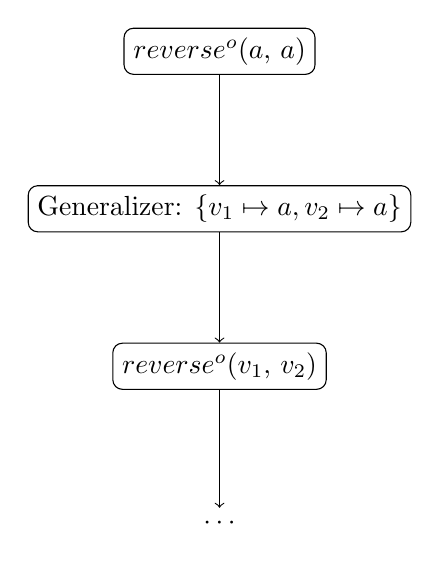
\begin{tikzpicture}[->,node distance=2cm, sibling distance=5cm]

\tikzstyle{conf}=[rectangle,draw, rounded corners=.8ex]
\node[conf] (root) {\relo{reverse}($a$, $a$)} ;
\node[conf] (gen) [below of = root] {Generalizer: $\{ v_1 \mapsto a, v_2 \mapsto a \}$};
\node[conf] (node) [below of = gen] {\relo{reverse}($v_1$, $v_2$)};
\node (rest)[below of = node] {$\cdots$};
\path (root) edge (gen)
      (gen) edge (node)
      (node) edge (rest);
\end{tikzpicture}
\caption{Демонстрация потери информации при обобщении вверх.}
\label{fig:genup}
\end{figure}

C одной стороны, теряется потенциал для генерации более оптимальной для цели \relo{reverse}($a$, $a$)
программы, но c другой стороны рассмотрим следующие соображения.

В данном примере процесс прогонки происходил следующим образом: некоторое время строился
граф для конфигурации \relo{reverse}($a$, $a$), затем вывелась конфигурация \relo{reverse}($a$, $b$).
Если бы обобщения вверх не происходило бы, то поиск ответов в результирующей программе
малое время провёл бы в поддереве, оптимизированном под \relo{reverse}($a$, $a$), а остальное --- в обобщённом
\relo{reverse}($a$, $b$).

В общем случае это может происходить не только с корнем дерева, но и в каких-то его поддеревьях.
Однако запрет на обобщение вверх в поддеревьях может сгенерировать слишком много частных случаев
и привести к более неэффективным программам.

Из того, что, во-первых, есть потенциал оптимизации при сохранении информации в корне дерева и,
во-вторых, необходимо сдерживать разрастание дерева конфигураций,
допускается рассмотрение алгоритма с обобщением вверх с запретом на обобщение к корню дерева.

%%%%%%%%%%%%%%%%%%%%%%%%%%%%%%%%%%%%%%%%%%%%%%%%%%%%%%%%%%%%%%%%%%%%%%%%%%%%%%
%%%%%%%%%%%%%%%%%%%%%%%%%%%%%%%%%%%%%%%%%%%%%%%%%%%%%%%%%%%%%%%%%%%%%%%%%%%%%%
%%%%%%%%%%%%%%%%%%%%%%%%%%%%%%%%%%%%%%%%%%%%%%%%%%%%%%%%%%%%%%%%%%%%%%%%%%%%%%
%%%%%%%%%%%%%%%%%%%%%%%%%%%%%%%%%%%%%%%%%%%%%%%%%%%%%%%%%%%%%%%%%%%%%%%%%%%%%%

\subsubsection{Расширение \ukanren оператором неэквивалентности}

Множество операций в оригинальном \ukanren покрывает все нужды реляционного программирования,
однако на ряде программ оно вычислительно допускает пути исполнения, которые не приводят
к успеху, однако сообщить об этом не представляется возможным.

К примеру, на рисунке~\ref{fig:lookup} изображена операция поиска значения по ключу
в списке пар ключ-значения \relo{lookup}.

\begin{figure}[h!]
\begin{lstlisting}
$\text{lookup}^o$ K L R =
   (K', V) :: L' $\equiv$ L $\land$
   (K' $\equiv$ K $\land$ V $\equiv$ R $\lor$ $\text{lookup}^o$ K L' R)
\end{lstlisting}
\caption{Отношения поиска значения по ключу.}
\label{fig:lookup}
\end{figure}

В соответствии с программой список \lstinline{L} должен иметь в голове пару из ключа и значения \lstinline{(K', V)}
и либо  этот ключ \lstinline{K'} унифицируется с искомым ключом \lstinline{K} и
значение \lstinline{V} --- с результатом \lstinline{R},
либо поиск происходит в хвосте списка \lstinline{L'}. Проблема этой программы в том,
что если унификация \lstinline{(K',V)::L' $\equiv$ L} прошла успешно и был
найден результат, то поиск всё равно продёт во вторую ветку с рекурсивным вызовом и будет
искать значение дальше, хотя по прагматике поиска ключа в списке должен вернуться лишь одно значение.
Более того, суперкомпилятору тоже придётся учитывать и, возможно, проводить вычисления,
которые не принесут никакой пользы.

В miniKanren существует операция неэквивалентности $t_1 \not\equiv t_1$, вводящая
ограничение неэквивалентности \origin{disequality contraints}\cite{mkConstr}.
Операция неэквивалентности определяет, что два терма $t_1$ и $t_2$ никогда не должны быть равны,
накладывая ограничения на возможные значения свободных переменных терма.

Расширение синтаксиса \ukanren представлено на рисунке~\ref{fig:syntaxExt}.

\begin{figure}[h!]
\centering
\[\begin{array}{ccll}
\mathcal{G}   & = & \hspace{1cm} \dots & \\
              &   & \hspace{1cm} \mathcal{T_X}\not\equiv\mathcal{T_X} \hspace{2cm} &\mbox{неэквивалентность} \\
\end{array}\]
\caption{Расширение синтаксиса \ukanren относительно указанного на рисунке~\ref{fig:syntax}.}
\label{fig:syntaxExt}
\end{figure}

Исправленная версия отношения \relo{lookup} представлена на рисунке~\ref{fig:lookupExt}.

\begin{figure}[h!]
\begin{lstlisting}
$\text{lookup}^o$ K L R =
   (K', V) :: L' $\equiv$ L $\land$
   (K' $\equiv$ K $\land$ V $\equiv$ R $\lor$
    K' $\not\equiv$ K $\land$ $\text{lookup}^o$ K L' R)
\end{lstlisting}
\caption{Исправленное отношение поиска значения по ключу.}
\label{fig:lookupExt}
\end{figure}

В такой реализации две по сути исключающие друг друга ветви исполнения будут исключать друг друга
и при вычислении запросов, и при суперкомпиляции.

Для реализации ограничения неэквивалентности вводится новая сущность под названием
``хранилище ограничений'' $\Omega$ \origin{constraints store}, которое используется для проверки
нарушений неэквивалентности. Окружение расширяется хранилищем ограничений, которое затем используется
при унификации и при добавлении новых ограничений.

Тогда нужно ввести следующие модификации в алгоритм унификации конфигурации, который собирает все
операции унификации в конъюнкции перед тем, как добавить её в множество допустимых конфигураций.
\begin{itemize}
\item При встрече операции неэквивалентности $t_1 \not\equiv t_2$ необходимо произвести следующие действия.
      Применить накопленную подстановку к термам $t_1 \theta = t_1'$ и $t_2 \theta = t_2'$ и
      унифицировать термы $t_1'$ и $t_2'$. Если получился пустой унификатор, значит, эти термы
      равны и ограничение нарушено. В таком случае суперкомпилятор покинет эту
      ветвь вычислений. Если же термы не унифицируются, значит, никакая подстановка
      в дальнейшем не нарушит ограничение. Иначе необходимо запомнить унификатор в хранилище.
\item При встрече операции унификации $t_1 \equiv t_2$ необходимо получить их унификатор.
      Если его не существует или он пуст, то дополнительных действий производить не нужно.
	  Иначе нужно проверить, не нарушает ли унификатор ограничения неэквивалентности.
\end{itemize}

Указанное расширение было добавлено в библиотеку с реализацией сопуствующих алгоритмов.

% Выявление остаточной программы по дереву процессов --- \emph{резидуализация} ---
% породит новые опеределения отношений. Больше одного отношения из дерева процессов может
% появиться в случае, когда узлы \lstinline{Renaming} указывают на узлы, отличные от корня.
% Поэтому первой фазой происходит пометка узлов, задающих таким образом отношения,
% а также удаление поддеревьев, у которых все ветви вычисления пришли к неудаче.

% Далее происходит обход дерева, во время которого генерируются узлы синтаксического дерева программы
% в зависимости от типа текущего узла дерева процессов:
% \begin{itemize}
% \item \lstinline{Unfoldable} узел приводит к появлению дизъюнкций подпрограмм, которые задают дети этого узла.
%       Это обусловлено тем, что при прогонке в этом узле происходит ветвеление вычислений;
% \item \lstinline{Abstraction} узел приводит к появлению конъюнкций подпрограмм, которые задают дети этого узла.
% 	  Это обусловлено тем, что хотя операция обобщения выявляет подконъюнкции из конфигурации и рассматривает их отдельно,
% 	  оба поддерева, задающиеся этими подконъюнкциями, должны выполнятся в одно и то же время;
% \item \lstinline{Generalizer} задаёт обобщающий унификатор, который должен быть добавлен
%       перед своим поддеревом;
% \item \lstinline{Renaming} формирует вызов реляционного отношения;
% \item \lstinline{Success} представляет собой успешное вычисление, предоставляющее непротиворечивую подстановку.
% \end{itemize}



\section{Экспериментальное исследование}
\label{sec:testing}

\subsection{Тестовое окружение}

В качестве основной конкретной реализации \ukanren для тестирования
использовался OCanren\footnote{Проект OCanren: \url{https://github.com/JetBrains-Research/OCanren}, дата последнего посещения: 15.05.2020}\cite{ocanren},
реализованный на OCaml\cite{ocanren}.
%Для некоторых тестов для использовался faster-miniKanren\footnote{\url{https://github.com/miniKanren/faster-miniKanren}},
%версия miniKanren, реализованная на Scheme.

Тесты запускались на ноутбуке со следующими характеристиками: Intel Core i5-6200U CPU, 2.30GHz, DDR4, 12GiB.

Для тестирования суперкомпилятора и его модификаций использовался следующий алгоритм.
\begin{enumerate}
\item Подготавливается программа, реализованная на внутреннем представлении $\mu$Kanren.
\item Программа и запрос, на который будет происходить специализация, подаются на вход суперкомпилятору.
\item По дереву процессов, порождённому суперкомпилятором, строится остаточная программа.
\item Остаточная программа транслируется в OCanren и
      запускается в заранее подготовленном окружении с тестовыми запросами.
\end{enumerate}


Реализованный суперкомпилятор сравнивался с реализацией \forcpd для $\mu$Kanren\footnote{Проект: \url{https://github.com/kajigor/uKanren_transformations}, дата последнего посещения: 15.05.2020},
а также c реализацией \forcpd для Prolog --- системой ECCE\footnote{Проект ECCE: \url{https://github.com/leuschel/ecce}, дата последнего посещения: 15.05.2020}.
Другие специализаторы не рассматриваются, так как согласно работе~\cite{controlPoly}, специализация с
помощью \forcpd в ECCE показывает лучшие результаты.

Для использования последнего требовалось оттранслировать программу на \ukanren в Prolog, специализировать
её на запрос, далее оттранслировать результирующую программу в OCanren.
Это допустимо сделать в силу того, что между \ukanren и чистым подмножеством Prolog есть
взаимно однозначное синтаксическое соответствие.
Все необходимые средства для этого также предоставлялись указанной библиотекой специализации.


\subsubsection{Набор тестов}

Был выбран следующий набор тестов для тестирования и анализа суперкомпилятора и его модификаций.
\begin{itemize}
 \item Программа \lstinline{doubleAppend(xs, ys, zs, rs)}, которая
       производит конкатенацию трёх списков. Она классически используется
       для проверки эффекта дефорестации в специализированной программе.
       Специализация происходила на запрос \lstinline{doubleAppend} со свободными переменными.
 \item Программа \lstinline{maxLength(xs, max, len)}, которая находит в списке
       максимальный элемент и длину списка. Она классически используется
       для проверки эффекта таплинга в специализированной программе.
       Специализация происходила на запрос \lstinline{maxLength} со свободными переменными.
 \item Программа сортировки \lstinline{sort(list, result)}. Выбрана в силу показательности
       результатов.
       Специализация происходила на запрос \lstinline{sort} со свободными переменными.
%     Запросы:
%     \begin{itemize}
%     \item оптимизация сортировки: \rel{sort}(xs, ys);
%     \item генерация отсортированных последовательностей: \rel{sort}(xs, xs).
%     \end{itemize}
 \item Отношение, проверяющее принадлежность пути графу \\
       \lstinline{isPath(path, graph, result)}.
       Специализация происходила на запрос \lstinline{isPath(path, graph, True)}.
       Запросы к программе для тестирования:
       \begin{itemize}
       \item поиск пути заданного размера в случайном графе: \\
       \lstinline{isPath(path, graph, True)$\land$length(path, N)};
       \item поиск фиксированного количества путей, принадлежащих данному графу.
       %\\ $\text{isPath}^o_s$(p, g)$\land$\rel{length}(p, N).
       \end{itemize}

	   В приложении А на рисунке~\ref{fig:graphGen} представлен код, который
	   был использован для генерации графов. Функции на вход
	   подаётся количество вершин, количество рёбер и зерно для генератора случайных чисел.
	   В тестах приводятся три графа на 20 вершинах с 50 рёбрами
	   с зёрнами: граф 1 --- 42, граф 2 --- 34, граф 3 --- 106.

 \item Интерпретатор формул логики высказываний \\ \lstinline{logint(formula, subst, result)}.
       Интерпретатор специализируется на то, чтобы всегда генерировать выполнимые формулы
       \lstinline{logint(formula, subst, True)}.
%      Запросы:
%     \begin{itemize}
%     \item поиск $n$ решений заданной формулы;
%     \item генерация $n$ формул с подстановке размера $n$.
%     \end{itemize}
 \item Интерпретатор лямбда-исчисления \lstinline{lam(expr, result)}.
       Интерпретатор специализируется на выражение \lstinline{lam(expr, result)}
       и используется для генерации $n$ выражений в нормальной форме \lstinline{lam(expr, expr)};
 	%\item генерация $n$ выражений, редуцирующихся к заданному выражению \lstinline{lam(expr, E)}.
 \item Проверка типов в просто типизировнном лямбда-исчислении \lstinline{infer(typ, expr)}.
%   \begin{itemize}
% 	\item Поиск $n$ обителей заданного типа.
% 	\item
     Отношение использовалось для генерация выражений, соответствующих заданной спецификации типа и выржения.
     Специализируется выражение:\\
 	 %\rel{infer}(type, expr) $\land$ type $\equiv$ TYPE\_SPEC $\land$ expr $\equiv$ EXPR\_SPEC.
 	 \lstinline{infer(typ, expr)$\land$typ $\equiv$ TYPE_SPEC$\land$expr $\equiv$ EXPR_SPEC}
 %  \end{itemize}
% \item Интерпретатор простого подмножества Scheme.
%    \begin{itemize}
%    \item \todo{Интересный тест!}
%    \end{itemize}
\end{itemize}

% Все вышеперечисленные программы были применены к реализованным суперкомпиляторами,
Ко всем вышеперечисленным программам были применены суперкомпиляторы,
и результаты выполнения остаточных программ были проверены на адекватность и соответствие задачам исходных программ.
Проводилось 10 измерений, пока которым выводились средние значения.
Следует отметить, что задачи доказательства сохранения семантики суперкомпилятором на стояло.

\subsection{Пример работы базового суперкомпилятора \ukanren}
% Для начала разберём, как базовый суперкомпилятор ведёт себя на
% базовом наборе программ, результат которых несложно проанализировать.

% \begin{itemize}
% \item Классическая программа \lstinline{doubleAppend}~\cite{cpd}, которая используется для
%       проверки наличия эффекта дефорестации (\todo{В приложении}).
% %\item Другая классическая программа \lstinline{maxLength}~\cite{cpd}, которая
% %      используется для проверки наличия эффекта таплинга.
% \end{itemize}

Разберём на примере результат работы базового суперкомпилятора.

Классическая программа для тестирования эффектов специализации ---
\lstinline{doubleAppend}, представленная на рисунке~\ref{fig:dappCode},
в которой происходит конкатенация списков трёх списков.

\begin{figure}[h!]
\begin{lstlisting}
doubleAppend a b c d =
  fresh (t)
   (append a b t $\land$ append t c d)
append y4 y5 y6 =
  (y4 $\equiv$ [] $\land$ y6 $\equiv$ y5) $\lor$
  fresh (ty t h)
   (y4 $\equiv$ h :: t $\land$
    y6 $\equiv$ h :: ty $\land$
    append t y5 ty)
\end{lstlisting}
\caption{Программа для тестирования \lstinline{doubleAppend}}
\label{fig:dappCode}
\end{figure}

Во многих бенчмарках~\cite{cpdPract, controlPoly} это программа используется
для проверки эффекта дефорестации.

Рассмотрим дерево процессов на рисунке~\ref{fig:dappTree}
(для компактности \lstinline{append} сокращён до \lstinline{app}),
которое порождается применением базового
суперкомпилятора к программе \lstinline{doubleAppend}, причём в
качестве аргументов --- простые свободные переменные, из-за чего
просто оптимизируется сама структура программы.

\begin{figure}[h!]
\center
\begin{minipage}[h]{\textwidth}
  \begin{tikzpicture}[->,node distance=1.2cm, sibling distance=5cm, level distance=2cm]
    \tikzstyle{conf}=[rectangle,draw, rounded corners=.8ex,align=center]
    \node[conf] (root) {{\it Unfolding} \\ \lstinline{doubleAppend(a, b, c, abc)}};
    \node[conf, below=of root] (appapp) {{\it Unfolding} \\ \lstinline{app(a, b, $\text{v}_0$)$\land$app($\text{v}_0$, c, abc)}};
    \node[conf, below=of appapp] (app1) {{\it Unfolding} \\ \lstinline{app($\text{v}_1$, c, $\text{v}_2$)} \\ $\{$ a $\mapsto$ [], b $\mapsto$ $\text{v}_0$, \\ $\text{v}_0 \mapsto \_ : \text{v}_1$, \\ $\ \ $ abc $\mapsto \_ : \text{v}_2$ $\}$};
    \node[conf, right=of app1] (app2) {{\it Renaming} \\ \lstinline{app($\text{v}_5$, b, $\text{v}_6$)$\land$}\\\lstinline{app($\text{v}_6$, c, $\text{v}_7$)} \\ $\{$ a $\mapsto \text{h} : \text{v}_5$ \\ $\text{v}_0 \mapsto \text{h} : \text{v}_6 $ \\ abc $\mapsto \text{h} : \text{v}_7$  $\}$};
    \node[conf, left=of app1] (appS) {{\it Success} \\ $\{$ a $\mapsto$ [], \\ \ \ b $\mapsto$ [],\\ \ \ $\text{v}_0 \mapsto$ [], \\ \ \ c $\mapsto$ abc $\}$};
    \node[conf, below right=of app1, anchor=north] (app11) {{\it Renaming} \\ \lstinline{app($\text{v}_3$, c, $\text{v}_4$)} \\ $\{\text{v}_1 \mapsto \_ : \text{v}_3 $ \\ $\ \ \ \ \text{v}_2 \mapsto \_ : \text{v}_4 $  $\}$};
    \node[conf, below left=of app1, anchor=north] (app1S) {{\it Success} \\ $\{ \text{v}_1 \mapsto [],$ \\ $\ \ c \ \mapsto \text{v}_2 \}$};
    \draw[-latex] (root) -- (appapp);
    \draw[-latex] (appapp) -- (appS.north);
    \draw[-latex] (appapp) -- (app1);
    \draw[-latex] (appapp) -- (app2);
    \draw[-latex] (app1) -- (app1S);
    \draw[-latex] (app1) -- (app11);
    \draw[-latex,dashed] (app2) edge [bend right] (root);
    \draw[-latex,dashed] (app11) edge [bend right] (app1);
  \end{tikzpicture}
\end{minipage}
\caption{Дерево процессов для программы \lstinline{doubleAppend}}
\label{fig:dappTree}
\end{figure}

В приведённом дереве первым этапом происходит замена определения \lstinline{doubleAppend}
на его тело. Так как в определении нет дизъюнкий, получаем всего одну конфигурацию,
в которой операцией \lstinline{fresh} добавляется новая семантическая переменная $\texttt{v}_0$.
Далее происходит обработка конфигурации с более чем одним конъюнктом. Так как используется
полная стратегия развёртывания, каждая из конъюнкий раскрывается по определению и
рассматривается их дизъюнктивная нормальная форма, в которой всего четыре дизъюнкта,
один из которых не унифицируется, поэтому всего появляется только три конфигурации.
Эти конфигурации рассматривают несколько возможных значений переменных:
\begin{enumerate}
\item когда \lstinline{a} и \lstinline{b} пустые списки, то результатом конкатенации
является \lstinline{c};
\item если же \lstinline{b} не пуст, тогда результат --- это конкатенация списков \lstinline{b} и \lstinline{c}.
      Отношение конкатенации двух списков также специализируется под задачу.
      В результате этой специализации порождается исходное отношение, поскольку
      никакой новой информации не было выявлено и исходная программа уже была оптимальна;
\item в третьем же случае выводится, что результат конкатенации трёх списков
      \lstinline{a}, \lstinline{b} и \lstinline{c} --- это конкатенация
      списков $\texttt{v}_5$, \lstinline{b} и \lstinline{c}, где $\texttt{v}_5$
      является хвостом списка, а в голову которой добавили голову \lstinline{a}.
\end{enumerate}

По данному дереву порождается остаточная программа, изображённая на рисунке~\ref{fig:dappCodeOpt}.
\begin{figure}[h!]
\begin{lstlisting}
doubleAppendo a b c d =
  fresh (x4) (app3 a b x4 c d)
app3 a b t c d =
   fresh (x7 x6 x5 x10 x9 x8)
     (a $\equiv$ [] $\land$ b $\equiv$ t $\land$
       (t $\equiv$ [] $\land$ c $\equiv$ d $\lor$
       (t $\equiv$ x8 :: x9) $\land$
        d $\equiv$ x8 :: x10 $\land$
        app2 x9 c x10
     ) $\lor$
     (a $\equiv$ x5 :: x6 $\land$
      t $\equiv$ x5 :: x7 $\land$
      d $\equiv$ x5 :: x10 $\land$
      app3 x6 b x7 c x10) )
app2 a b c =
  fresh (x13 x12 x11)
   (a $\equiv$ [] $\land$ b $\equiv$ c $\lor$
   (a $\equiv$ x11 :: x12 $\land$
    c $\equiv$ x11 :: x13 $\land$
    app x12 b x13))
\end{lstlisting}
\caption{Суперкомпилированная программа \lstinline{doubleAppend}}
\label{fig:dappCodeOpt}
\end{figure}

В итоге, наблюдается, как двупроходный алгоритм становится однопроходным.


\subsection{Сравнение вариаций суперкомпилятора \ukanren}

В таблицах используются условные обозначения для стратегий развёртывания:
\begin{itemize}
\item {\it Full} и {\it Full-non-rec} обозначают полную стратегию и полную стратегию развёртывания с приоритетом на нерекурсивные вызовы соответственно;
\item {\it Seq} обозначает последовательную стратегию развёртывания;
\item {\it Non-rec} и {\it Rec} обозначают нерекурсивную и рекурсивную стратегии соответственно;
\item {\it Min} и {\it Max} обозначают минимальную и максимальную стратегии соответственно;
\item {\it First} обозначает стратегию, при которой всегда развёртывается первый конъюнкт.
\end{itemize}

А также для суперкомпиляторов:
\begin{itemize}
\item {\it Б.С.} обозначает базовый суперкомпилятор с обобщением вниз на предков;
\item {\it М.1 } обозначает модификацию, при которой происходит запрет на обобщение сразу после обобщения;
\item {\it M.2 } обозначает модификацию, при которой обобщение происходит на все ранее вычисленные вершины;
\item {\it M.3 } обозначает модификацию, при которой происходит обобщение вверх на родительские вершины;
\item {\it M.4 } обозначает модификацию, при которой происходит обобщение вверх на родительские вершины, кроме корневой.
\item {\it M.5 } обозначает модификацию, при которой происходит обобщение вверх на родительские вершины, а также запрет обобщения после обобщения.
\end{itemize}


В таблице~\ref{fig:dappTest} представлены результаты сравнения модификаций
с базовым суперкомпилятором при разных стратегиях развёртывания.
При полных стратегиях для \lstinline{doubleAppend} возникает эффект дефорестации.
В остальных стратегиях этого не происходит, из-за чего исполнения по
крайней мере в два раза хуже. Из-за того, что программа довольно небольшая,
модификации алгоритма суперкомпиляции хотя не и оказывают влияния, результат не ухудшают.

\begin{table}[h!]
\center
\begin{tabular}{|l|c|c|c|c|c|c|}
\hline
                   &{\it Б.С.}&{\it М.1}&{\it М.2}&{\it М.3}&{\it M.4} & {\it M.5} \\ \hline
%Original: 0.010374
%ECCE: 0.004058
%CPD: 0.012664
{\it Full        }& {\bf 0.0049}  & 0.0055       & 0.0056       & {\bf 0.0050} & {\bf 0.0048} & 0.0053\\ \hline
{\it Full-non-rec}& 0.0053        & {\bf 0.0048} & {\bf 0.0049} & {\bf 0.0050} & {\bf 0.0037} & {\bf 0.0039} \\ \hline
{\it Seq         }& 0.0098        & 0.0119       & 0.0099       & 0.0127       & 0.0097       & 0.0102 \\ \hline
{\it Non-rec     }& 0.0100        & 0.0122       & 0.0099       & 0.0099       & 0.0097       & 0.0098 \\ \hline
{\it Rec         }& 0.0094        & 0.0133       & 0.0103       & 0.0098       & 0.0097       & 0.0100 \\ \hline
{\it Min         }& 0.0096        & 0.0122       & 0.0100       & 0.0093       & 0.0094       & 0.0099 \\ \hline
{\it Max         }& 0.0096        & 0.0096       & 0.0092       & 0.0101       & 0.0119       & 0.0091 \\ \hline
{\it First       }& 0.0120        & 0.0094       & 0.0094       & 0.0099       & 0.0093       & 0.0093 \\ \hline

\end{tabular}
\caption{Результат для \lstinline{doubleAppendo} c конкатенацией трёх списков длины 120, секунды}
\label{fig:dappTest}
\end{table}

В таблице~\ref{fig:maxlenTest} указаны результаты выполнения для
программы \lstinline{maxLength} на списке \lstinline{[1..200]}.

\begin{table}[h!]
\center
\begin{tabular}{|l|c|c|c|c|c|c|}
\hline
                  &{\it Б.С.}   &{\it М.1}      &{\it М.2}      &{\it М.3}&{\it M.4} & {\it M.5}\\ \hline
%Orig: 0.270905
%ECCE: 0.230436
%CPD: 0.653551
{\it Full        } & 0.623        & 0.638       & {\bf 0.250}  & {\bf 0.250} & {\bf 0.251} & 0.293 \\ \hline
{\it Full-non-rec} & 0.633        & 0.611       & 0.602        & 0.256       & 0.258 & 0.298 \\ \hline
{\it Seq         } & 0.285        & 0.290       & 0.289        & 0.289       & 0.287 & 0.286 \\ \hline
{\it Non-rec     } & 0.284        & 0.289       & 0.285        & 0.285       & 0.287 & 0.287 \\ \hline
{\it Rec         } & 0.856        & 0.893       & 0.560        & 0.577       & 0.569 & 0.888 \\ \hline
{\it Min         } & 0.317        & {\bf 0.280} & 0.303        & 0.284       & 0.279 & {\bf 0.280} \\ \hline
{\it Max         } & {\bf 0.279}  & 0.287       & 0.279        & 0.278       & 0.284 & 0.281 \\ \hline
{\it First       } & 0.864        & 0.858       & 0.564        & 0.963       & 0.949 & 0.565 \\ \hline


\end{tabular}
\caption{Запуск для \lstinline{maxLength} на списке \lstinline{[1..200]}, секунды}
\label{fig:maxlenTest}
\end{table}

Модификация алгоритма {\it M.2-M.4} на стратегии {\it Full} породили программы
с эффектов таплинга, при котором максимальный элемент и длина списка высчитывались
за один проход. Интересное наблюдение состоит в том, что в других случаях, к примеру,
при применении стратегии {\it Seq}, таплинга не происходит, но сама программа
исполняется не существенно медленнее.

В таблице~\ref{fig:sortTest} указаны результаты тестирования для
программы \lstinline{sort} при сортировки списков случайного содержания (числа от 0 до 50)
длины 50.

\begin{table}[h!]

\center
\begin{tabular}{|l|c|c|c|c|c|c|}
\hline
                  &{\it Б.С.}&{\it М.1}&{\it М.2}&{\it М.3}&{\it M.4}&{\it M.5}\\ \hline
{\it Full        } & {\bf 0.239} & 0.252       & {\bf 0.238} & {\bf 0.232} & {\bf 0.239} & 0.244 \\ \hline
{\it Full-non-rec} & 0.241       & {\bf 0.240} & 0.241       & 0.241       & 0.245       & {\bf 0.242} \\ \hline
{\it Seq         } & 0.242       & {\bf 0.240} & {\bf 0.239} & 0.238       & {\bf 0.240} & 0.254 \\ \hline
{\it Non-rec     } & 0.245       &  0.242      & 0.247       & {\bf 0.236} & 0.244       & {\bf 0.242} \\ \hline
{\it Rec         } & 0.239       &  0.242      & 0.252       & 0.240       & 0.250       & 0.243 \\ \hline
{\it Min         } & 0.245       & 0.252       & 0.242       & 0.242       & 0.292       & 0.279 \\ \hline
{\it Max         } & 0.246       & 0.242       & 0.249       & 0.246       & 0.246       & 0.239 \\ \hline
{\it First       } & 0.250       & 0.248       & 0.263       & 0.245       & 0.239       & 0.247 \\ \hline


\end{tabular}
\caption{Запуск для \lstinline{sort}, секунды}
\label{fig:sortTest}
\end{table}

Примечательно, что на всех списках указанного свойства алгоритмы отработали практически
одинаково. Более примечательно, что какие бы модификации ни взяли,
порождаются довольно схожие программы. Это обосновывается тем, что само отношение
сортировки имеет весьма короткое рекурсивное определение.

В таблицах~\ref{fig:logintTest1},~\ref{fig:logintTest2} и~\ref{fig:logintTest3} указаны результаты тестирования для
программы \lstinline{logint}, которая использовалась для генерации всех выполнимых формул
без свободных переменных, с одной свободной переменной и с двумя свободными переменными соответственно.

\begin{table}[h!]
\center
\begin{tabular}{|l|c|c|c|c|c|c|}
\hline
   &{\it Б.С.}&{\it М.1}&{\it М.2}&{\it М.3}&{\it M.4}&{\it M.5}\\ \hline
{\it Full        } &    -        &    -         & 0.132       &  0.105       &    -        & -     \\ \hline
{\it Full-non-rec} & {\bf 0.076} & 0.072        & 0.210       &  0.111       & 0.126       & {\bf 0.081} \\ \hline
{\it Seq         } & 0.168       & 0.181        & 0.149       &  0.090       & {\bf 0.091} & 0.113 \\ \hline
{\it Non-rec     } & 0.078       & 0.092        & 0.136       &  0.088       & 0.114       & 0.099 \\ \hline
{\it Rec         } & 0.081       & 0.074        & {\bf 0.095} &  {\bf 0.064} & 0.126       & 0.090 \\ \hline
{\it Min         } & 0.080       & {\bf 0.064}  & 0.110       &  0.092       & 0.117       & 0.082 \\ \hline
{\it Max         } & 0.164       & 0.193        & 0.144       &  0.077       & 0.111       & 0.146 \\ \hline
{\it First       } & 0.181       & 0.164        & 0.176       &  0.070       & 0.189       & 0.136 \\ \hline
\end{tabular}
\caption{Запуск \lstinline{logint} для генерации формул без переменных, секунды.}
\label{fig:logintTest1}
\end{table}

\begin{table}[h!]
\center
\begin{tabular}{|l|c|c|c|c|c|c|}
\hline
   &{\it Б.С.}&{\it М.1}&{\it М.2}&{\it М.3}&{\it M.4}&{\it M.5} \\ \hline
{\it Full        }&    -         &     -        & 0.078       & 0.068       &    -        &  -  \\ \hline
{\it Full-non-rec}& 0.056        &  0.045       & 0.125       & 0.084       & 0.082       & 0.051\\ \hline
{\it Seq         }& 0.109        &  0.110       & 0.086       & 0.063       & 0.074       & 0.069 \\ \hline
{\it Non-rec     }& {\bf 0.046}  &  {\bf 0.038} & 0.081       & 0.072       & {\bf 0.067} & {\bf 0.045} \\ \hline
{\it Rec         }& 0.055        &  0.050       & 0.074       & {\bf 0.055} & 0.079       & 0.055\\ \hline
{\it Min         }& 0.053        &  0.041       & {\bf 0.066} & {\bf 0.055} & 0.079       & 0.059\\ \hline
{\it Max         }& 0.100        &  0.117       & 0.108       & 0.057       & 0.074       & 0.077\\ \hline
{\it First       }& 0.118        &  0.103       & 0.091       & 0.068       & 0.101       & 0.084\\ \hline
\end{tabular}
\caption{Запуск \lstinline{logint} для генерации формул с одной переменной, секунды.}
\label{fig:logintTest2}
\end{table}

\begin{table}[h!]
\center
\begin{tabular}{|l|c|c|c|c|c|c|}
\hline
   &{\it Б.С.}&{\it М.1}&{\it М.2}&{\it М.3}&{\it M.4}&{\it M.5} \\ \hline
{\it Full        }&    -        &    -        & 0.078       & 0.062      &    -        & - \\ \hline
{\it Full-non-rec}& 0.137       & 0.040       & 0.093       & 0.042      & 0.069       & {\bf 0.040} \\ \hline
{\it Seq         }& 0.086       & 0.082       & 0.066       & 0.049      & {\bf 0.050} & {\bf 0.041} \\ \hline
{\it Non-rec     }& 0.043       & {\bf 0.031} & 0.063       & 0.044      & 0.055       & 0.046 \\ \hline
{\it Rec         }& {\bf 0.037} & 0.034       & {\bf 0.045} & 0.040      & 0.051       & 0.049 \\ \hline
{\it Min         }& {\bf 0.037} & 0.039       & 0.049       & 0.041      & 0.054       & 0.045 \\ \hline
{\it Max         }& 0.068       & 0.070       & 0.067       &{\bf 0.036} & 0.062       & 0.071 \\ \hline
{\it First       }& 0.104       & 0.100       & 0.110       & 0.095      & 0.137       & 0.073 \\ \hline
\end{tabular}
\caption{Запуск \lstinline{logint} для генерации формул с двумя переменными, секунды.}
\label{fig:logintTest3}
\end{table}

Прочерки в таблицах обозначают то, что из-за большой требовательности к ресурсам,
на тех модификациях, которые не приводят к быстрому сворачиванию программ,
включая и базовый суперкомпилятор, не удалось получить оптимизированные программы.
Однако ожидается,
что при должном количестве ресурсов порождённые программы окажутся слишком большими,
что приведёт к значительным проблемам производительности, из-за чего добиваться
результатов
для данных случаев в данной работе считается нецелесообразным.

В представленных таблицах наблюдается, что при увеличении количества свободных переменных,
в среднем, уменьшается время генерации формул. Это обосновывается тем, что в
деревьях исполнения порождаемых программам больше ветвей оканчиваются успешным
поиском значения в подстановке.



\subsubsection{Исследование модификации с ограничением неэквивалентности}

Для исследования влияния ограничения неэквивалентности рассматривается отношение
интерпретатора лямбда-исчисления \lstinline{lam}, с помощью которого
происходил поиск 50-ти термов в нормальной форме.

В таблице~\ref{fig:lamTestSimple} приведено время выполнения программы
без введения ограничения неэквивалентности. Здесь наблюдается интересная закономерность:
на очередном интерпретаторе модификации {\it M.1} и {\it M.5} показывают лучшие результаты.

\begin{table}[h!]
\center
\begin{tabular}{|l|c|c|c|c|c|c|}
\hline
   &{\it Б.С.}&{\it М.1}&{\it М.2}&{\it М.3}&{\it M.4}&{\it M.5} \\ \hline

{\it Full        } & {\bf 0.106}& 0.088     & 0.102       & 0.106       & 0.095       & 0.084 \\ \hline
{\it Full-non-rec} & {\bf 0.106}& 0.086     & 0.111       & 0.105       & {\bf 0.083} & 0.082 \\ \hline
{\it Seq         } & 0.107      & 0.085     & 0.105       & {\bf 0.103} & {\bf 0.083} & {\bf 0.080} \\ \hline
{\it Non-rec     } & 0.112      & 0.087     & 0.{\bf 100} & 0.110       & 0.086       & 0.084 \\ \hline
{\it Rec         } & 0.111      &{\bf 0.083}& 0.112       & 0.111       & 0.090       & 0.083 \\ \hline
{\it Min         } & 0.109      & 0.095     & 0.110       & 0.114       & 0.093       & 0.085 \\ \hline
{\it Max         } & 0.107      & 0.098     & 0.105       & 0.105       & 0.086       & 0.086 \\ \hline
{\it First       } & {\bf 0.106}& 0.089     & 0.111       & 0.118       & 0.093       & 0.092 \\ \hline
\end{tabular}
\caption{Запуск \lstinline{lam} для поиска термов в нормальной форме без оператора неэквивалентности, секунды.}
\label{fig:lamTestSimple}
\end{table}

В таблице~\ref{fig:lamTestDiseqSimple} указано время исполнения на программе с
использованием оператора неэквивалентности только в отношении подстановки, которое
используется интерпретатором.

\begin{table}[h!]
\center
\begin{tabular}{|l|c|c|c|c|c|c|}
\hline
   &{\it Б.С.}&{\it М.1}&{\it М.2}&{\it М.3}&{\it M.4}&{\it M.5} \\ \hline

{\it Full        } & {\bf 0.040} &  0.025    & 0.052     &0.046      & 0.024     & 0.024 \\ \hline
{\it Full-non-rec} & 0.042       &  0.025    & 0.042     &0.044      & 0.024     & 0.025 \\ \hline
{\it Seq         } & 0.044       &  0.026    & 0.046     &0.045      &{\bf 0.022}& 0.027 \\ \hline
{\it Non-rec     } & {\bf 0.040} &  0.026    & 0.046     &0.042      & 0.025     &{\bf 0.022} \\ \hline
{\it Rec         } & 0.045       &{\bf 0.023}&{\bf 0.041}&0.044      & 0.027     &{\bf 0.022} \\ \hline
{\it Min         } & 0.042       &  0.034    & 0.045     &0.045      & 0.023     & 0.027 \\ \hline
{\it Max         } & 0.043       &  0.026    & 0.043     &{\bf 0.040}& 0.027     & 0.028 \\ \hline
{\it First       } & 0.044       &  0.027    & 0.045     &0.042      & 0.025     & 0.023 \\ \hline
\end{tabular}
\caption{Запуск \lstinline{lam} для поиска термов в нормальной форме с оператором неэквивалентности, секунды.}
\label{fig:lamTestDiseqSimple}
\end{table}

Из таблицы виден прирост производительности для методов {\it М.1}, {\it M.4} и
{\it M.5} практически в четыре раза, а для остальных -- в два. \\

% Однако оператор можно использовать и для реализации самого интерпретатора при
% определении, является ли левая часть аппликации лямбда-теромом.
%
% \begin{table}[h!]
% \center
% \begin{tabular}{|l|c|c|c|c|c|c|}
% \hline
%                   &{\it Б.С.}  &{\it М.1}  &{\it М.2}  &{\it М.3}  &{\it M.4}  &{\it M.5} \\ \hline
% {\it Full        }&0.050       &  0.042    & 0.052     & 0.048     & 0.037     & 0.041 \\ \hline
% {\it Full-non-rec}&0.048       &  0.048    & 0.050     & 0.047     & 0.038     & 0.041 \\ \hline
% {\it Seq         }&{\bf 0.046} &{\bf 0.036}& 0.048     &{\bf 0.046}& 0.039     & 0.038 \\ \hline
% {\it Non-rec     }&0.049       &  0.041    & 0.049     & 0.049     & 0.042     &{\bf 0.036} \\ \hline
% {\it Rec         }&0.049       &  0.042    & 0.050     & 0.048     & 0.041     &{\bf 0.036} \\ \hline
% {\it Min         }&{\bf 0.046} &  0.040    & 0.045     & 0.047     & 0.037     & 0.037 \\ \hline
% {\it Max         }&0.051       &  0.038    &{\bf 0.044}& 0.048     &{\bf 0.036}& 0.042 \\ \hline
% {\it First       }&0.049       &  0.044    & 0.049     & 0.049     & 0.042     & 0.041 \\ \hline
% \end{tabular}
% \caption{Запуск \lstinline{lam} для поиска термов в нормальной форме c оператором неэквивалентности, секунды.}
% \label{fig:lamTestDiseq}
% \end{table}

% Несмотря на то, что разные подходы на разных классах программ показывают
% себя с лучшей стороны, в среднем модификация с обобщением вверх при
% нерекурсивной стратегии развёртывания показывает себя лучше всего.

Разные подходы показывают себя хорошо на разных классах задач.
При этом стабильно самой неудачной стратегией развёртки себя
показывает стратегия {\it First}. Самыми неудачными модификациями оказались
{\it M.1} и {\it М.2}.
Модификация \textit{M.2} с обобщением на все рассмотренные вершины стабильно приводит
к слишком раннему сворачиванию дерева, из-за чего теряется точность специализации.
Модификация \textit{M.1}, наоборот, делает слишком много развёртываний, что также
приводит к потере производительности.
В целом, смена стратегии базового суперкомпилятора позволила увеличить
производительность большинства порождаемых программ. В среднем, лучше
всего работают стратегии \textit{Seq} и её модификация \textit{Non-rec}.
Реализация обобщения вверх \textit{M.3} значительно улучшила производительность программ.
Её модификация \textit{M.4} выигрывала в больших случаях, однако периодически
значительно проигрывает, как и модификация \textit{M.5}, которая хорошо показала
себя только на интерпретаторах.

В итоге, оптимальной модификацией считается суперкомпилятор с обобщением
вверх с нерекурсивной стратегией развёртывания.


\subsection{Сравнение суперкомпилятора с существующими решениями}

В таблице~\ref{fig:totalResult} представлены результаты сравнения базового алгоритма
суперкомпиляции ({\it Б.С,}) и выбранной наиболее успешной модификации
суперкомпилятора ({\it М.С.}) с оригинальными программами ({\it Оригинал}),
а также с оптимизированными программами с помощью
системы ECCE для Prolog с использованием трансляции ({\it ECCE}) и адаптации
конъюнктивной частичной дедукции для miniKanren ({\it CPD}).

\begin{table}[h!]
\center
\begin{tabular}{|c|c|c|c|c|c|}
\hline
{\it Параметр} & {\it Оригинал} & {\it ECCE }  & {\it CPD} & {\bf Б.C} & {\bf М.С.} \\ \hline
{\bf doubleAppend} & \multicolumn{5}{|l|}{списки фиксированной длины } \\ \hline
120                & 0.0135 & 0.0051 & 0.0133 & {\bf 0.0049} & 0.0098 \\ \hline


{\bf maxLength} & \multicolumn{5}{|l|}{фиксированный список} \\ \hline

       [1..200] & 0.257 & {\bf 0.230} & 0.727 & 0.623 & 0.287 \\ \hline


%\rowcolor{black!10}
{\bf sort} & \multicolumn{5}{|l|}{случайный список фиксированной длины } \\ \hline
50       & 8.42     & 12.28 & 13.2 & 0.239  & {\bf 0.242} \\ \hline

%\rowcolor{black!10}
 {\bf isPath} & \multicolumn{5}{|l|}{10 путей} \\ \hline
  граф 3      & > 300 & {\bf 1.03} & 1.19 & 2.43 & 1.81 \\ \hline

 {\bf isPath} & \multicolumn{5}{|l|}{произвольный путь длины 7} \\ \hline
   граф 3     & 62.12 & 1.08 & 1.15 & 1.34 & {\bf 0.85} \\ \hline
 {\bf isPath} & \multicolumn{5}{|l|}{произвольный путь длины 10} \\ \hline
 граф 1  &  12.51  & 1.01 & 1.20 &  1.28 & {\bf 0.48} \\
 граф 2  &  > 300s & 1.73 & 2.09 & 0.85 & {\bf 0.48} \\
 граф 3  &         & 9.90 & 12.73& 3.29 & {\bf 1.23} \\
 \hline

%\rowcolor{black!10}
{\bf logint} & \multicolumn{5}{|l|}{размер подстановки} \\ \hline
0 & > 300    & 0.17  & 2.7  & -  &  {\bf 0.11} \\
1 &          & 0.09  & 1.7  & -  &  {\bf 0.07} \\
2 &          & 0.08   & 0.9  & -  & {\bf 0.05} \\
\hline

%\rowcolor{black!10}
{\bf lam} & \multicolumn{5}{|l|}{термы в нормальной форме} \\ \hline
%10 термов к себе    & 0.17     & 0.001 & 0.008 & 0.002  \\
50 термов & > 300    & 2.98  & 0.08 & 0.08 & {\bf 0.04}   \\
%1000 термов к const & 1.01     & 0.126 & 0.263 & 0.274  \\
\hline
% {\bf scheme} & \multicolumn{5}{|l|}{программы, сводящиеся к const} \\ \hline
% 41 терм      &
{\bf genBySpec} & \multicolumn{5}{|l|}{генерация по спецификации} \\ \hline
2000            & > 300 & 0.53 & 0.62 & - & {\bf 0.36} \\ \hline
\end{tabular}
\caption{Результаты сравнения алгоритмов специализации, cекунды}
\label{fig:totalResult}
\end{table}

В случае с \lstinline{doubleAppend}, которому на вход подали три одинаковых списка длины 120,
базовому суперкомпилятору удалось
добиться эффекта дефорестации и сравниться с {\it ECCE}, модифицированный суперкомпилятор
уступает {\it ECCE}, однако всё ещё быстрее как оригинальной программы, так и {\it CPD}.

Однако в тесте \lstinline{maxLength}, которому на вход подали список [1..200], базовый суперкомпилятор пусть и делает
таплинг, но добавляет ветвистости программе, из-за чего она работает хуже оригинальной
почти в два раза, однако модифицированный алгоритм пусть не ускоряет исполнение программы,
ухудшает её незначительно, в отличие от {\it CPD}. Стоит заметить, что ECCE пусть и
улучшил производительность, отличие от оригинальной программы оказалось несущественным.

Исполнение программы сортировки \lstinline{sort} на случайном списке длины 50 и элементами
не более 50, в свою очередь, заметно ускорилось относительно и оригинала, и специализированных
программ с помощью конъюнктивной частичной дедукции. Это может объясняться тем, что в некоторых
случаях методы конъюнктивной частичной дедукции делают лишние развёртывания, что в конечном
счёте приводит к ухудшению программы.

Отношение проверки принадлежности пути графу \lstinline{isPath} использовалось
для поиска 10 путей в указанном графе. Здесь результат работы суперкомпиляции
проиграл примерно в два раза алгоритмам конъюнктивной частичной дедукции,
но решил задачу значительно быстрее оригинала. Однако уже на более
осмысленной задаче по поиску путей заданной длины суперкомпилятор
значительно выиграл у методов конъюнктивной частичной дедукции.


Также был рассмотрен интерпретатор логических формул \lstinline{logint}, который
запускался для поиска формул и их подстановок, в которой они выполняются, для
формул с нулём, одним и двумя свободными переменными. Это пример запуска в ``обратную''
сторону, который, как можно наблюдать из таблицы, действительно крайней неэффективен.
Специализированные же версии дают значительный прирост производительности, однако
модифицированная версия суперкомпилятора выигрывает у всех методов. Прочерки стоят,
как объяснялось в предыдущем подразделе, из-за того, что в данном случае стратегия
полного развёртывания требовала слишком много ресурсов.

В примере с отношением \lstinline{lam} базовый суперкомпилятор отработал
идентично \textit{CPD}, но модифицированный в два раза быстрее нашёл 50 термов
в нормальной форме.

Довольно сложным примерном для суперкомпилятора оказалось отношение
по генерации термов по спецификации:
\begin{itemize}
\item спецификация терма: \lstinline{app (app _ _) _};
\item спецификация типа: \lstinline{_ $\to$ (_ $\to$ not-arrow _)}.
\end{itemize}

% Полная стратегия развёртки базового компилятора вновь не справилась,
% но модификация значительно выигрывает у оригинала и опять побеждает методы
% конъюнктивной частичной дедукции.
Суперкомпиляция с полной стратегией развертки вновь не уложилась в имеющиеся ограничения
на ресурсы, однако модифицированная версия значительно повышает эффективность программы,
даже относительно \textit{ECCE} и \textit{CPD}.

%По результатам экспериментального исследования можно сделать вывод,
%что разработанный суперкомпилятор в среднем показывает хорошие результаты
%и на большинстве рассмотренных программ даёт значительный прирост производительности,
%как относительно оригинальной программы, так и относительно рассмотренных
%методов специализации.


\phantomsection
\section*{Заключение}
\addcontentsline{toc}{section}{ЗАКЛЮЧЕНИЕ}

В результате проделанной работы был разработан суперкомпилятор для miniKanren,
реализованы его модификации, а также произведено их экспериментальное исследование.

Реализованный суперкомпилятор показал улучшение производительности на подавляющем
большинстве рассмотренных программ относительно исходной программы, а также относительно
реализаций конъюнктивной частичной дедукции;
в иных случаях проблемы с производительностью оказывались несущественными.

Исходный код проекта можно найти на сайте \url{https://github.com/RehMaar/uKanren-spec},
автор принимал участие под учётной записью RehMaar.

Результаты работы были представлены на конференции TEASE-LP'20.



\renewcommand{\refname}{Список использованных источников}
% \printbibliography

\renewcommand{\refname}{Приложение A}
\section*{Приложение А}

%\begin{figure}[h!]
%\begin{lstlisting}
%doubleAppend z1 z2 z3 z4 =
%  (z1 $\equiv$ nil () $\land$ app3 z2 z3 z4) $\lor$
%  fresh (fE fB fA)
%    (z1 $\equiv$ fA :: fB $\land$
%    (z4 $\equiv$ fA :: fE) $\land$
%    appD fB z2 z3 fE)
%
%appD z1 z2 z3 z4 =
%  (z1 $\equiv$ nil ()  $\land$ app3 z2 z3 z4) $\lor$
%  fresh (fE fB fA)
%   (z1 $\equiv$ fA :: fB $\land$
%   (z4 $\equiv$ fA :: fE) $\land$
%    appD fB z2 z3 fE)
%
%app3 z1 z2 z3 =
%  (z1 $\equiv$ nil () $\land$ (z2 $\equiv$ z3)) $\lor$
%  fresh (fD fC fB fA)
%    (z1 $\equiv$ fA :: fB $\land$
%    (z3 $\equiv$ fA :: fD) $\land$
%    app3 fB z2 fD)
%\end{lstlisting}
%\caption{Специализированная системой ECCE программа \lstinline{doubleAppend}}
%\end{figure}


\begin{figure}[h!]
\begin{lstlisting}[basicstyle=\scriptsize]{language=Haskell}
generateGraph :: Int -> Int -> Int -> [(Int, Int)]
generateGraph n m =
   evalRand (do tree <- forM [1..n-1] $\textdollar$ \i ->
                   getEdge i           <$\textdollar$>
                   getRandomR (0, i-1) <*>
                   getRandom
                rest <- replicateM (m - n + 1) $\textdollar$
                   getRandomR (0, n-2) >>=
                     \i -> getEdge i             <$\textdollar$>
                           getRandomR (i+1, n-1) <*>
                           getRandom
                pure $\textdollar$ tree ++ rest) . mkStdGen
    where getEdge :: Int -> Int -> Bool -> (Int, Int)
          getEdge i j True = (i, j)
          getEdge i j False = (j, i)
\end{lstlisting}
\caption{Генератор случайного ориентированного графа с заданными параметрами.}
\label{fig:graphGen}
\end{figure}


% \end{document}
